\section{Study 1. The Developmental Patterns of Pronoun Case Error}
\subsection{Corpora}
To avoid the limitation of small sample size and data selection bias, this study conducted a comprehensive corpus analysis of speech from monolingual English-speaking children from roughly ages two to four. That includes 46 children with longitudinal recordings in CHILDES. Table \ref{table:1} shows the summary of the corpus.
\begin{table}[h]
\footnotesize
\centering
\caption{Summary of Corpus Information} 
\label{table:1}
%\begin{adjustbox}
\begin{tabular}{l|l|l|l|l|l}
\toprule
\multicolumn{6}{c}{\textbf{North American Corpora}} &
\hline
\textbf{Corpora}  & \textbf{Child}  & \textbf{Age} &
\textbf{Corpora}  & \textbf{Child}  & \textbf{Age}\\
\hline
\cite{bloom1974imitation}  & Peter   & 1;9-3;2 & \cite{suppes1974semantics} &  Nina & 2;0-3;4
\\
\cite{braunwald1971mother}  & Laura   & 1;5-4;0 & \cite{kuczaj1978children} &  Abe & 2;5-4;0 \\
\multirow{}{}*{\cite{brown1973first}} & Adam & 2;3-4;0 & \cite{demetras1986working} & Trevor & 2;1-4;0\\
& Eve & 1;6-2;3 & \multirow{}{}*{\cite{Weist2009}} & Ben & 2;4-3;4 \\
& Sarah & 2;3-4;0 & &Emily & 2;6-3;4\\
\cite{demetras1989changes} & Jimmy & 2;2-2;10 & & Emma & 2;7-3;9\\
\cite{clark1978awareness} & Shem & 2;3-3;2 &  & Jilian & 2;1-2;10\\
\cite{sachs1983talking}& Naomi & 1;3-4;9 & & Matt & 2;5-5;0\\
\cite{macwhinney2014childes} & Ross & 1;4-5;0 & & Roman & 2;3-4;0\\
\multirow{}{}*{\cite{post1993language}}& She & 1;8-2;5 & \cite{Snow1990child} & Nathaniel & 3;1-3;3\\
&Tow&1;9-2;5&\cite{hayes1988vocabulary}&Geraldine&1;6-2;2\\
\hline
\hline
& \textbf{No.} & \textbf{Mean Age} & & \textbf{No.} & \textbf{Mean Age}\\
\cite{bates1991first}  & 11  & 2;4 &
\cite{bohannon1977children}  & 2 & 3;6\\
\cite{gleason1980acquisition}&19&4;8&\cite{snow1995shell}&79&3;11\\
\cite{snow1989imitativeness}&25&2;8&\cite{valian1991syntactic}&17&2;5\\
\cite{van1980effects}&19&3;9\\
\hline
\hline
\multicolumn{6}{c}{\textbf{UK Corpora}}&
\hline
\textbf{Corpora}  & \textbf{Child}  & \textbf{Age} &
\textbf{Corpora}  & \textbf{Child}  & \textbf{Age}\\
\hline
\multirow{}{}*{\cite{henry1995belfast}} & Barbara & 2;4-4;1 & \multirow{}{}*{\cite{theakston2001}} & Anne & 1;10-2;9\\
& Michelle & 2;4-4;4 & & Warren& 1;10-2;9 \\
& Courtney & 3;4-4;0 & &Aran & 1;11-2;10\\
 & Rachel & 2;5-3;2 & & Becky & 2;0-2;11\\
 & Conor & 3;8-4;5 &  & Carl & 1;8-2;8\\
& Stuart & 3;5-4;5 & & Dominic & 1;10-2;10\\
 & Johnny & 3;5-4;4 & & Gail & 1;11-2;11\\
 & David & 2;0-4;2 &  & Joel & 1;11-2;10\\
\cite{rowland2006effect} & Lara & 1;9-3;3&  & John &1;11-2;10 \\
\cite{maslen2004dense} & Thomas & 2;0-4;11 & & Liz& 1;11-2;10\\
\multirow{}{}*{\cite{lieven2009two}} &Eleanor &2;0-3;1 & & Nicole& 2;0-3;0 \\
&Fraser &2;0-3;0 & & Ruth& 1;11-2;11 \\
\hline
\hline
&\textbf{No.}&\textbf{Mean Age}& &\textbf{No.}&\textbf{Mean Age}\\
\cite{tommerdahl2013analyzing}&23&2;9&\cite{howe1981acquiring}&16&2;0\\
\hline
\bottomrule
\end{tabular}
%\end{adjustbox}
\end{table}

This study applied the \textsc{nltk} python package to automatically extract data from the annotated corpora in CHILDES. The data that has been collected from each child's file include their age, mlu, total number and parents' input words, total number of sentences and input sentences, total number of each pronoun and each input pronoun. 

\subsection{Finding Errors}
The annotated \texttt{.xml} files were used to search for errors. CHILDES applies MOR and GRASP programs to annotate part-of-speech tags and dependency grammatical relations for all the transcripts. For English data, the automated annotation system has been reported to have high-level accuracies: the MOR program reaches 97\% of accuracy and the GRASP program has 95.8\% accuracy for identifying the subjects and 94.1\% accuracy for identifying the objects \citep{macwhinney2012morphosyntactic,sagae2010morphosyntactic}. The MOR program produces the \texttt{\%mor} tier, in which part-of-speech tags stand in one-to-one correspondence with the word in the transcript line. The \texttt{\%mor} tier assigns \texttt{pro:sub} to the nominative pronouns, \texttt{pro:obj} to the objective pronouns and \texttt{det:poss} to the genitive pronouns. Case-ambiguous pronouns `you' and `it' are tagged as \texttt{pro:per} which doesn't differentiate their nominative use and objective use. Pronoun `her' is tagged as \texttt{pro:obj} when it is used as an object and \texttt{det:poss} when it is used as a determiner. The GRASP program produces the \texttt{\%gra} tier which represents grammatical relations. The \texttt{\%gra} assigns \texttt{SUBJ} for the word in the subject position,  \texttt{OBJ} or \texttt{POBJ} for the word in the object position, and \texttt{DET} for the word in the determiner position. The \texttt{\%mor} tier assigns the case (e.g. \texttt{pro:sub} or \texttt{pro:obj}) based on the pronoun itself, regardless of the context it is used in. The \texttt{\%gra} tier assigns the case based on the argument position, despite the pronoun's own case. An excerpt from Peter in Brown corpus in (\ref{example}) exemplifies the \texttt{\%mor} tier and \texttt{\%gra} tier. All the errors were first extracted using \texttt{nltk} python package \citep{bird2009natural}, and then hand-checked by two annotators independently. 
\begin{exe}
\ex \label{example} \gll *CHI: \textbf{you}'re getting vitamins for \textbf{me }.\\
\%mor:	\textbf{pro:per|you}~aux|be&PRES part|get-PRESP n|vitamin-PL prep|for \textbf{pro:obj|me} .\\
\%gra:\textbf{	1|3|SUBJ} 2|3|AUX 3|0|ROOT 4|3|OBJ 5|3|JCT \textbf{6|5|POBJ} 7|3|PUNCT\\
(\href{https://childes.talkbank.org/browser/index.php?url=Eng-NA/Bloom/Peter/020812.cha}{Bloom/Peter/020812.cha})
\end{exe}

\subsubsection{NOM case errors and OBJ case errors}
The NOM case errors are nominative cased pronouns used in the non-subject position, e.g. `she hit \textit{I}'. The OBJ case errors are objective cased pronouns used in the non-object position, e.g. `\textit{me} drink milk'. These two types of errors were located on \texttt{\%gra} tier, since \texttt{\%gra} tier identifies subject and object based on the the relationship between arguments. For nominative cased pronouns \textit{I, he, she, we, they}, if they appear in a sentence with dependency grammatical relations \footnote{Children produce many incomplete sentences and run-on sentences. Not all the incomplete sentences have dependency grammatical relations, such as \textit{`I yeah'} and \textit{`um I I I.'}. To have dependency grammatical relations, the sentence needs to have at least two words from different grammatical categories that can be combined together. Sentences without dependency grammatical relations are excluded in this study.} 
and if they are not tagged as \texttt{SUBJ} on the \texttt{\%gra} tier, it is counted as an error. For example, in sentence (\ref{meseehe}), the nominative cased pronoun \textit{`he'} is used in an object position and it is tagged as \texttt{OBJ} on the \texttt{\%gra} tier. In (\ref{hehat}), \textit{`they'} is tagged as \texttt{POBJ} (object) on the \texttt{\%gra} tier too. 
\begin{exe}
\ex \label{meseehe}\gll *CHI: when \textit{\textbf{me}} see \textit{\textbf{he}} again ?\\
\%mor: conj|when \textit{\textbf{pro:obj|me}} v|see \textit{\textbf{pro:sub|he}} adv|again ? \\
\%gra: 1|3|LINK \textbf{\textit{2|3|SUBJ}} 3|0|ROOT \textit{\textbf{4|3|OBJ}} 5|4|JCT 6|3|PUNCT \\
(\href{https://childes.talkbank.org/browser/index.php?url=Eng-NA/Brown/Eve/020100b.cha}{Brown/Eve/020100b.cha})
\ex \label{hehat}\gll *CHI: all of \textit{\textbf{they}} going go in here.\\
\%mor: pro:indef|all prep|of pro:sub|they part|go-PRESP~inf|to v|go prep|in n|here\\
\%gra: 1|0|INCROOT 2|1|NJCT 3|2|POBJ 4|3|XMOD 5|6|INF 6|4|COMP 7|6|JCT 8|7|POBJ 9|1|PUNCT.\\
(\href{https://childes.talkbank.org/browser/index.php?url=Eng-NA/Suppes/021021.cha}{Suppes/021021.cha})
\end{exe}
Similar to the searching process for the NOM case errors, for objective cased pronouns \textit{me, him, us, them}, if they appear in a sentence with dependency grammatical relations and if they are not tagged as \texttt{OBJ} or \texttt{POBJ}, they were counted as error. For example, in sentence (\ref{meseehe}) and (\ref{666}), \textit{me} is an objective cased pronoun and it was used as the subject, which was tagged as \texttt{SUBJ}. In sentence (\ref{meshoew}), \textit{me} is used as a determiner, which was tagged as \texttt{MOD}(modifier). In sentence (\ref{them}), \textit{them} is used as a determiner, but it was tagged as \texttt{SUBJ} on the \%gra tier. Although the tag is not correct, as long as it is not tagged as \texttt{OBJ} or \texttt{POBJ}, it is still counted as an error. The third person singular feminine pronoun \textit{her} is a special case, because it can be used as an object or a determiner. The \texttt{\%mor} tier is used to distinguish accusative \textit{her} and genitive \textit{her}. The former is tagged as \texttt{pro:obj} and the latter is tagged as \texttt{det:poss}. All the \textit{her}s that are not tagged as \texttt{OBJ} or \texttt{POBJ} or \texttt{DET} or \texttt{MOD} on the \texttt{\%gra} tier are counted as error. For example, in (\ref{herdidnt}) \textit{her} is tagged as \texttt{SUBJ} on the \texttt{\%gra} tier, thus counted as an error. 

All the NOM and ACC errors were first identified using \texttt{nltk} python package and hand checked by two annotators. 

\begin{exe}
\ex \label{666}\gll *CHI: \textit{\textbf{me}} come back.\\
\%mor: \textit{\textbf{pro:obj|me}} v|come adv|back .\\
\%gra: \textit{\textbf{1|2|SUBJ}} 2|0|ROOT 3|2|JCT 4|2|PUNCT. \\
(\href{https://childes.talkbank.org/browser/index.php?url=Eng-NA/Brown/Eve/011000a.cha}{Brown/Eve/011000a.cha})
\ex \label{meshoew} \gll *CHI:	where's \textbf{\textit{me}} shoes ?\\
\%mor:	pro:int|where~cop|be&3S \textit{\textbf{pro:obj|me}} n|shoe-PL ?\\
\%gra:	1|2|SUBJ 2|0|ROOT \textbf{\textit{3|4|MOD}} 4|2|PRED 5|2|PUNCT\\
(\href{https://childes.talkbank.org/browser/index.php?url=Eng-NA/Suppes/020228.cha}{Suppes/020228.cha})
\ex \label{them} \gll *CHI:	\textbf{\textit{them}} guys can beat up this guy .\\
\%mor:	\textit{\textbf{pro:obj|them}} n|guy-PL n|can n|beat adv|up det:dem|this n|guy .\\
\%gra:\textbf{\textit{	1|2|SUBJ} }2|4|MOD 3|4|MOD 4|0|ROOT 5|4|NJCT 6|7|DET 7|5|POBJ 8|4|PUNCT\\
(\href{https://childes.talkbank.org/browser/index.php?url=Eng-NA/Kuczaj/020700.cha}{Kuczaj/020700.cha})
\ex \label{herdidnt}\gll *CHI: \textit{\textbf{her}} didn't wanna.\\
\%mor: \textbf{\textit{det:poss|her}} mod|do&PAST~neg|not v|want~inf|to .\\
\%gra:	\textit{\textbf{1|4|SUBJ}} 2|4|AUX 3|2|NEG 4|0|ROOT 5|4|OBJ 6|4|PUNCT. \\
(\href{https://childes.talkbank.org/browser/index.php?url=Eng-NA/Brown/Eve/020300b.cha}{Brown/Eve/020300b.cha})
\end{exe}


\subsubsection{GEN case error}
Genitive case errors were not identified in the \texttt{\%gra} tier, since the \texttt{\%gra} tier is less successful in capturing phrasal relationship. The genitive cased pronouns are not always tagged as \texttt{SUBJ} or \texttt{OBJ} even when they appear in the subject or object position. For example in (\ref{mywantit}), the genitive case pronoun `\textit{my}' is in the subject position, but it is tagged as \texttt{DET} (determiner) on the \texttt{\%gra} tier. 

Instead, genitive case errors are located using \texttt{\%mor} tier by an exhaust search of all the impossible part-of-speech tag combinations that contain a determiner. Genitive cased pronouns could be mistakenly used as a subject or an object in the sentence. When a genitive cased pronoun is misused as a subject, it is likely to precede a verb; and when it is misused as an object, it is likely to appear after a verb. Therefore, when an genitive cased pronoun, \textit{my, his, our, their}, occurs with a verb, including past and present participles (in (\ref{got}) and (\ref{mywantit})) and auxiliaries (in (\ref{mycan}) and (\ref{his}), it is counted as an error. 

\begin{exe}
\ex \label{} \gll *CHI:	when \textit{\textbf{my}} take a nap. \\
\%mor:	conj|when \textit{\textbf{det:poss|my}} v|take det:art|a n|nap.\\
\%gra:	1|3|LINK 2|3|DET 3|0|ROOT 4|5|DET 5|3|OBJ 6|3|PUNCT.
\ex \label{got} \gll *CHI: yeah \textit{\textbf{my}} got.\\
\%mor: co|yeah \textit{\textbf{det:poss|my}} v|get&PAST.\\
\%gra: 1|3|COM \textit{\textbf{2|3|DET }} 3|0|ROOT.\\
(\href{https://childes.talkbank.org/browser/index.php?url=Eng-NA/Brown/Sarah/030018b.cha}{Brown/Sarah/030018b.cha})
\ex \label{mywantit} \gll  *CHI: what \textit{\textbf{my}}  doing?  \\     
\%mor:	pro:int|what \textit{\textbf{det:poss|my}} part|do-PRESP?\\
\%gra:	1|3|LINK \textit{\textbf{2|3|DET}} 3|0|ROOT 4|3|PUNCT\\
(\href{https://childes.talkbank.org/browser/index.php?url=Eng-NA/Brown/Eve/020100b.cha}{Brown/Eve/020100b.cha})
\ex \label{mycan} \gll *CHI: \textit{\textbf{my}} can sing.\\
\%mor: \textbf{\textit{det:poss|my}} mod|can v|sing.\\
\%gra: \textit{\textbf{1|3|DET}} 2|3|AUX 3|0|ROOT 4|3|PUNCT\\
(\href{https://childes.talkbank.org/browser/index.php?url=Eng-NA/Braunwald/010607.cha}{Braunwald/010607.cha})

\ex \label{his} \gll *CHI:	here \textit{\textbf{his}} is. \\
\%mor:	adv|here \textbf{\textit{det:poss|his}} cop|be&3S .\\
\%gra:	1|3|JCT 2|3|DET 3|0|ROOT 4|3|PUNCT\\
(\href{https://childes.talkbank.org/browser/index.php?url=Eng-NA/Suppes/021006.cha}{Suppes/021006.cha})
\ex \label{getdressed} \gll *CHI: get \textit{\textbf{my}} dressed now .\\
\%mor:	v|get \textit{\textbf{det:poss|my}} part|dress-PASTP adv|now .\\
\%gra:	1|0|ROOT \textit{\textbf{2|3|DET}} 3|1|COMP 4|3|JCT 5|1|PUNCT\\
(\href{https://childes.talkbank.org/browser/index.php?url=Eng-UK/Thomas/021105.cha}{Thomas/021105.cha})
\ex \label{bigpoop} \gll *CHI:	it's \textit{\textbf{my}} done a big poo in there . \\
\%mor:	pro:per|it~cop|be&3S \textit{\textbf{det:poss|my}} part|do&PASTP det:art|a adj|big n|poo prep|in n|there .\\
\%gra:	1|2|SUBJ 2|0|ROOT \textit{\textbf{3|4|DET}} 4|2|PRED 5|7|DET 6|7|MOD 7|4|OBJ 8|4|JCT	9|8|POBJ 10|2|PUNCT\\
(\href{https://childes.talkbank.org/browser/index.php?url=Eng-UK/Thomas/030010.cha}{Thomas/030010.cha})
\end{exe}


\subsubsection{Exclusion Criterion}
There are exceptions where an accusative pronouns can be used in the subject position. For example, conjoined subjects such as `\textit{Me and mommy} went shopping' are allowed and widely accept in English. However, the conjoined subjects were identified as errors with the \texttt{nltk} package, since the accusative in the conjoined subject are tagged as \texttt{SUBJ} on the {\%gra} tier, as shown in (\ref{conjoined}). Two annotators have hand checked all the error sentences and excluded conjoined subjects as errors. 

\begin{exe}
\ex \label{conjoined} \gll *CHI: an(d) \textbf{me} an(d) Papa buy some salt.\\
\%mor: coord|and \textbf{pro:obj|me} coord|and n:prop|Papa v|buy qn|some n|salt .\\
\%gra: 1|5|LINK \textbf{2|5|SUBJ} 3|2|CONJ 4|3|COORD 5|0|ROOT 6|7|QUANT 7|5|OBJ 8|5|PUNCT.\\
(\href{https://childes.talkbank.org/browser/index.php?url=Eng-NA/Brown/Eve/020300a.cha}{Brown/Eve/020300a.cha})
\end{exe}
Along with case errors, children also make many other types of errors involving pronouns. Those errors are not included in this study. In this study, the errors are strictly defined as case errors, which means that as long as the error can be corrected by only changing the case of the pronoun, it is counted as a case error. For example, (\ref{excl1}) is an error sentence with pronouns. However it doesn't count as a pronoun case error, since the problem of the sentence lies in the verb, which can not be resolved by replacing `\textit{I}' or/and `\textit{he}' with `\textit{me/my}' or/and `\textit{him/his}'. Similarly, sentence (\ref{wantme}) doesn't count as an error since \textit{I} and \textit{me} were correctly used as the subject and object in the sentence. 
\begin{exe}
\ex \label{excl1} \gll *CHI:	I dead him .\\
\%mor:	pro:sub|I adj|dead pro:obj|him .\\
\%gra:	1|3|SUBJ 2|3|MOD 3|0|INCROOT 4|3|PUNCT\\ 
(Fraser/020405a)
\ex \label{wantme} \gll *CHI: I want me read the other way. \\
\%mor: pro:sub|I v|want pro:obj|me v|read&ZERO det:art|the qn|other n|way.\\
\%gra: 1|2|SUBJ 2|0|ROOT 3|4|SUBJ 4|2|COMP 5|7|DET 6|7|QUANT 7|4|OBJ 8|2|PUNCT\\
(\href{https://childes.talkbank.org/browser/index.php?url=Eng-NA/Suppes/020228.cha}{Suppes/020228.cha})
\end{exe}

\subsection{Results}
\subsubsection{The Overall Rate of Pronoun Case Errors From Cross-sectional Data}
The overall rate of pronoun case errors were calculated based on 211 children with cross-sectional recordings. Among 211 children, 141 children didn't make any errors in their transcripts. The average pronoun case error rate is 1.16\%, with the maximum error rate of 31.79\%. The distribution of the pronoun case error rate is plotted in Figure \ref{fig:212}. Over 95\% of the children's pronoun case error rate is less than 5\%, suggesting that most children rarely make any pronoun case errors. In addition, 211 children has a wide age range from 1;10 - 5;2. It is possible that the children with high error rates are the younger ones. The distribution of age and average pronoun correct rate for each age points is plotted in Figure \ref{fig:cross}. The averaged pronoun correct rate for each age point ranges from 100\% to 96\%. The pronoun correct rate does not show a linear relationship with age; instead, it appears to be a U-shaped pattern, that the children start with almost perfect correct rate with about 99\% and drop to 96\% and rise back 99\% and 100\%. The U-shaped developmental pattern is widely observed in many areas of language development, such as phoneme discrimination \citep{werker1983developmental}, passive structure acquisition \citep{maratsos1974children} and past tense overregularization errors \citep{marcus1992overregularization, plunkett1993rote, jackson1997attention}. The U-shaped pattern is very interesting since it provides insights of the underlying process of pronoun case acquisition. The longitudinal data needs to be examined to confirm if there is the U-shaped pattern in pronoun case errors too. In conclusion, the cross-sectional data suggests that the pronoun case error is a relatively rare phenomenon that displays a U-shaped development pattern. 

\FloatBarrier
\begin{figure}[h]
\centering
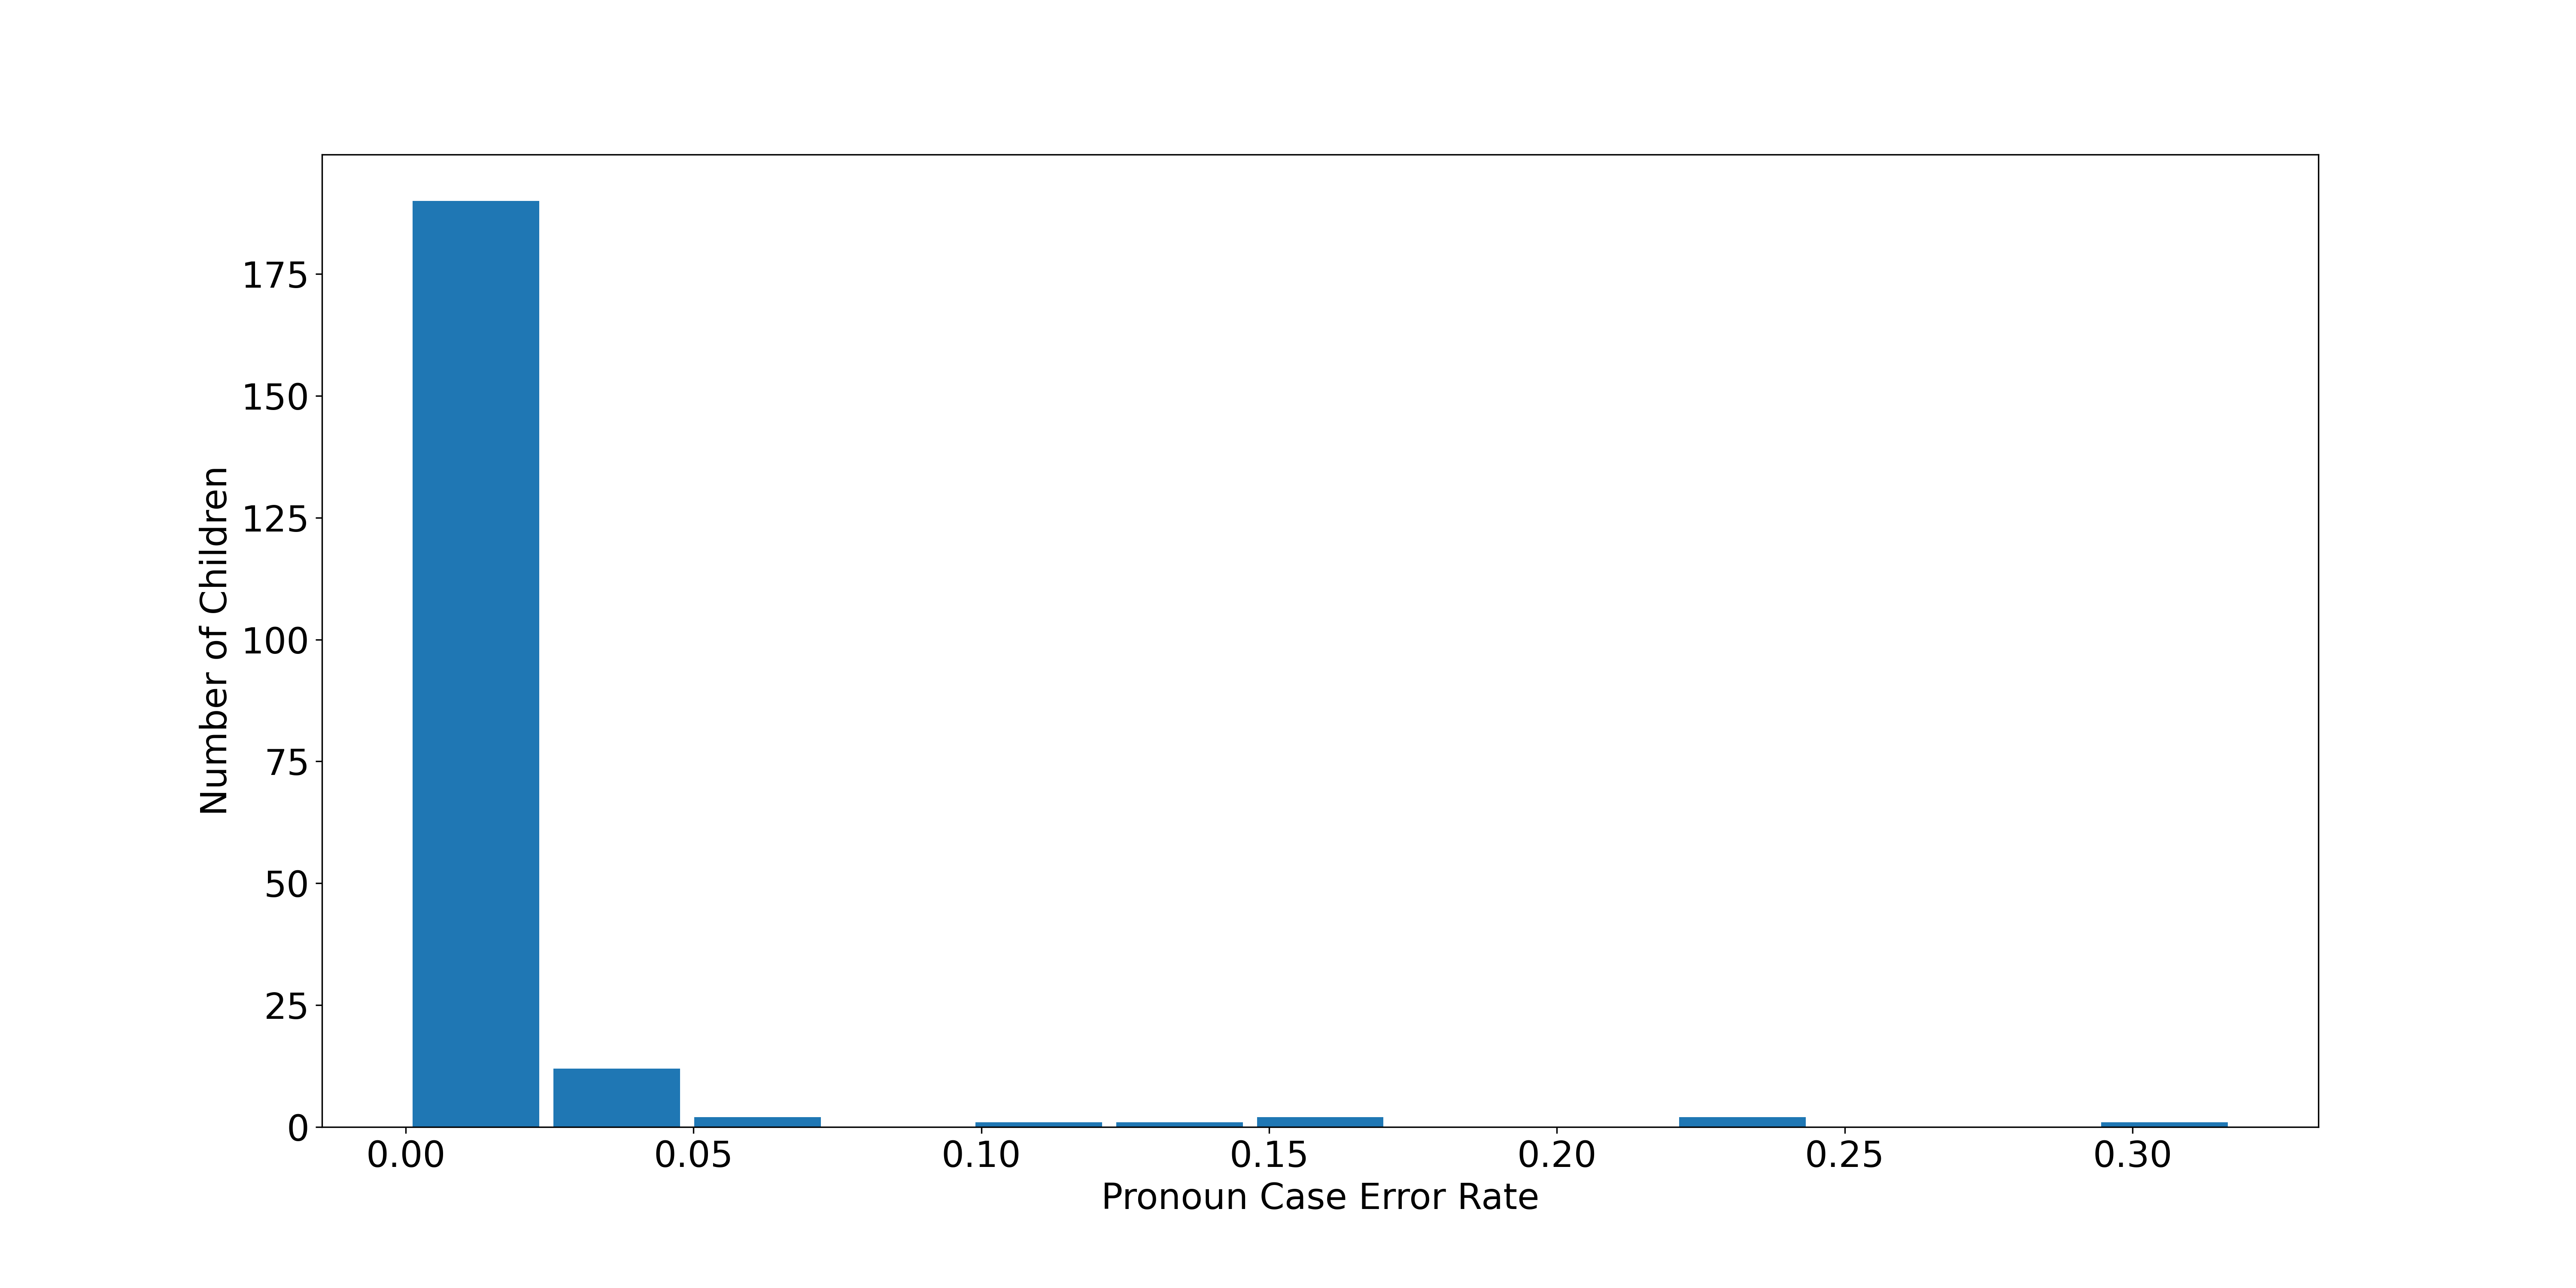
\includegraphics[scale = 0.35]{graph/OverallErrorRate.png}
\vspace{-3em}
\caption{Histogram of pronoun case error rate among 211 children}
\label{fig:212}
\end{figure}
\FloatBarrier
\begin{figure}[h]
\centering
    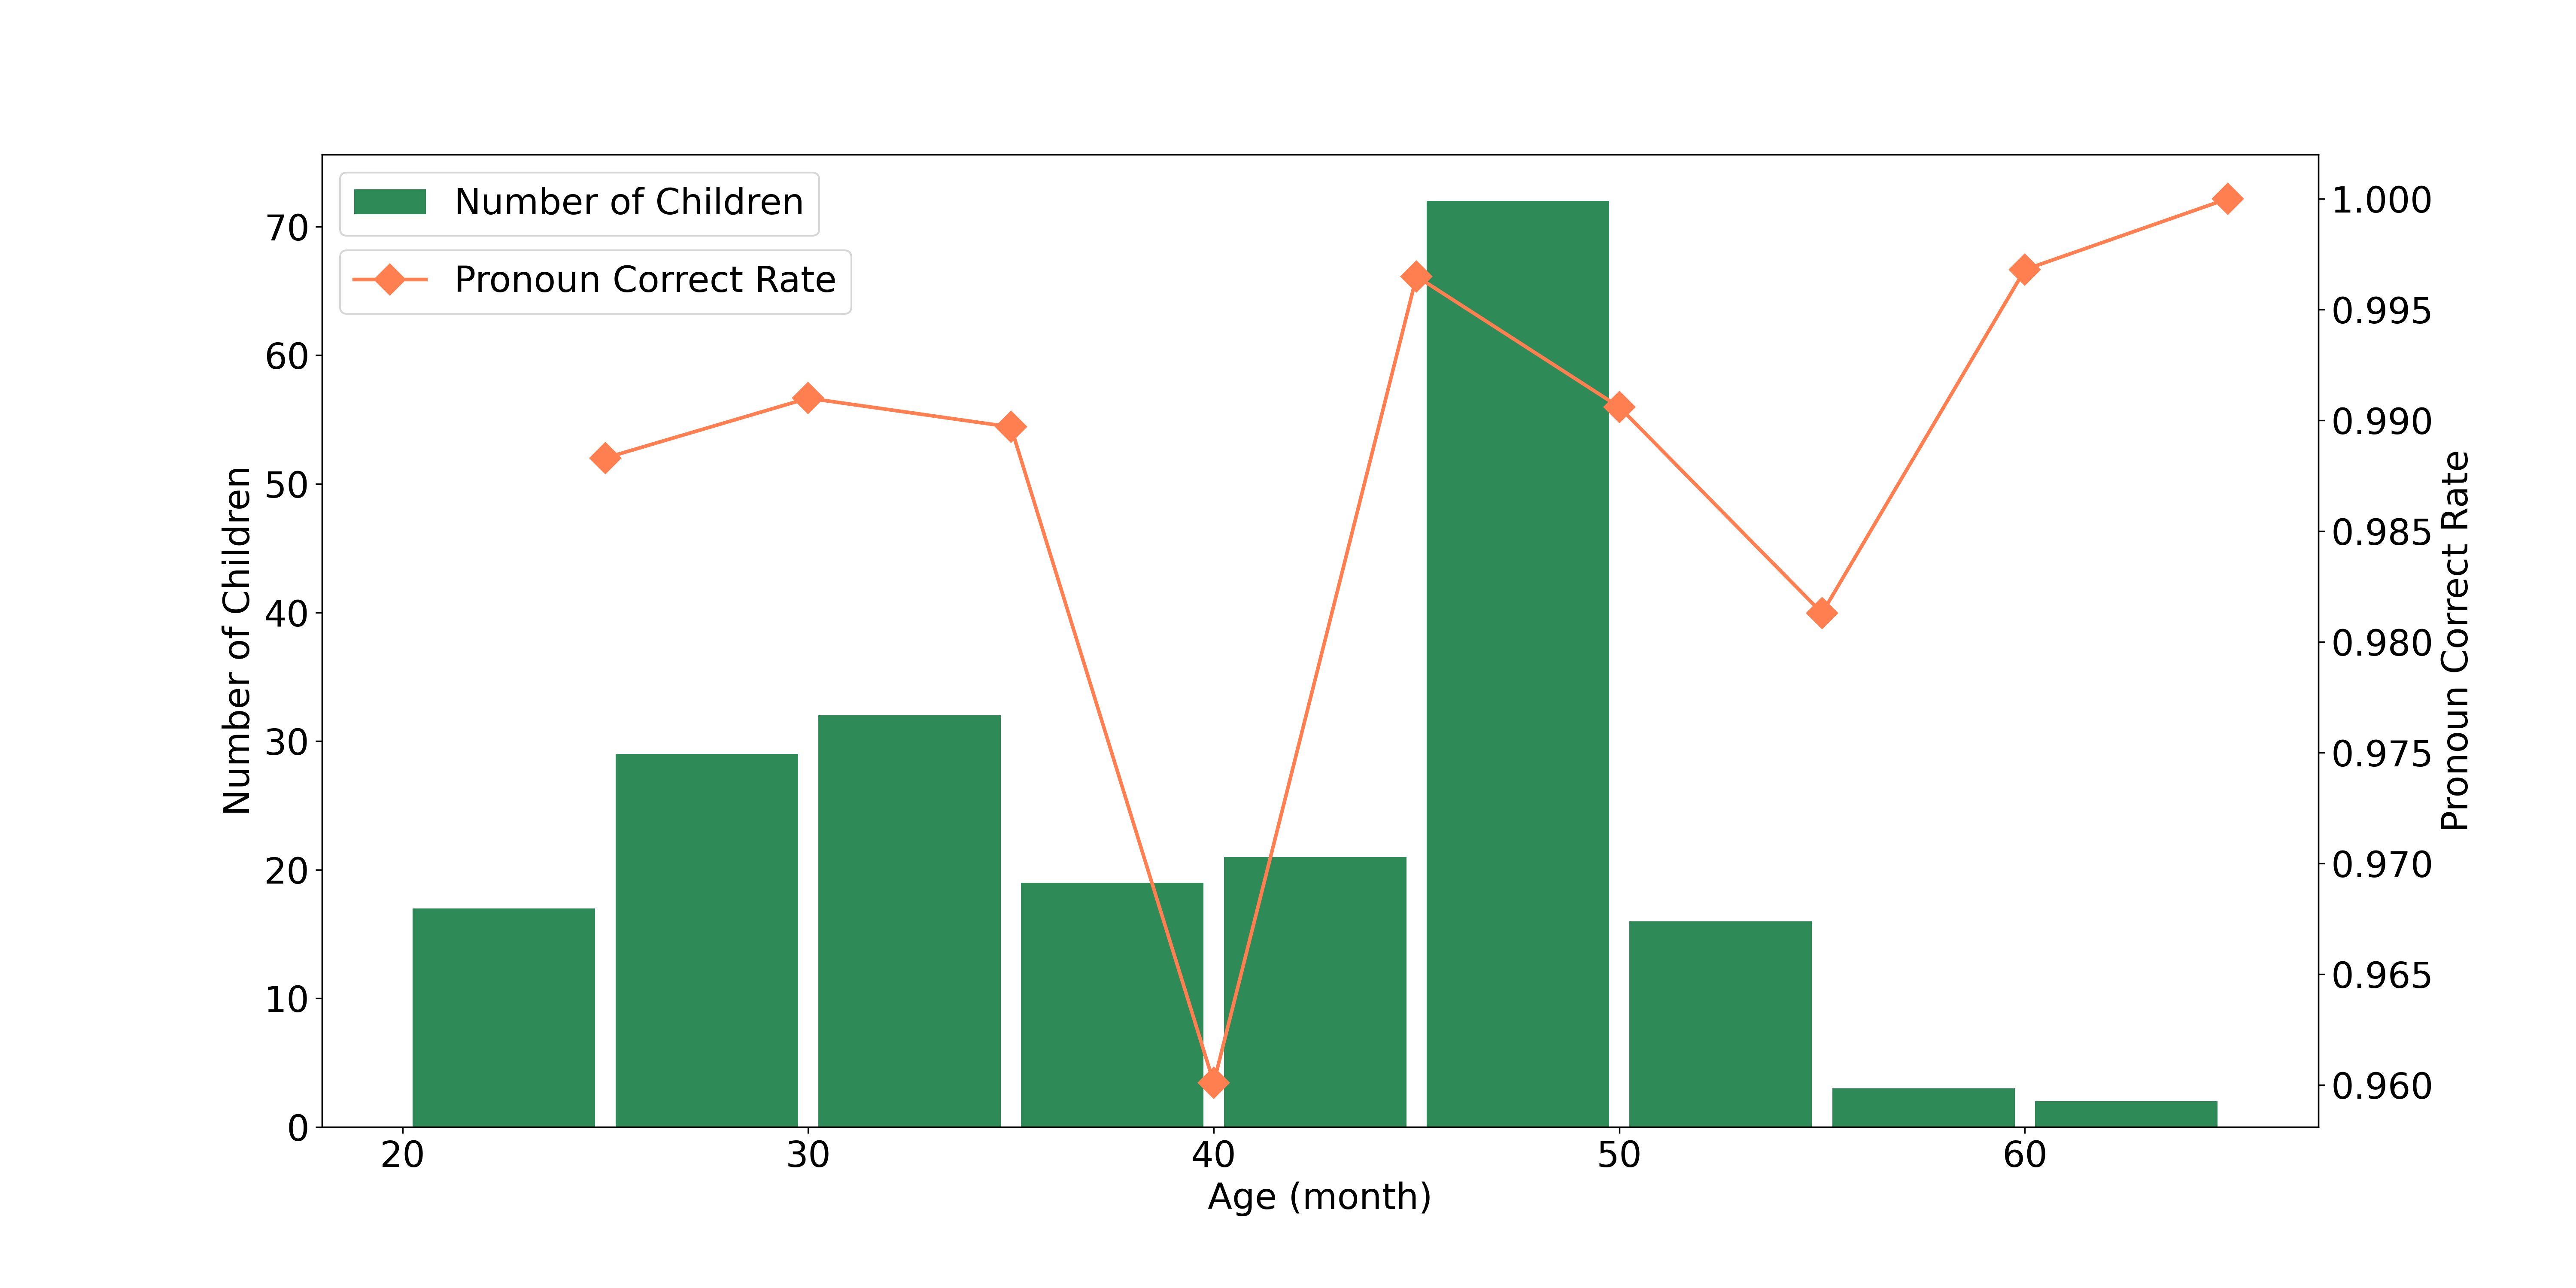
\includegraphics[scale =0.35] {graph/Crosssectional.png}
    \vspace{-3em}
    \caption{Histogram of Age with Pronoun Correct Rate}
    \label{fig:cross}
\end{figure}
\subsubsection{The Rate of Pronoun Case Errors from Longtitudinal Data}
Table \ref{table:2} shows a summary of each longitudinal child's total number of pronouns production, total number of pronoun input and total number of pronoun case errors with age and mlu range. The average correct rate is 98.44\% and the median correct rate is 99.40\%, suggesting that most of the children rarely make any  pronoun case errors. 

In order to examine if there's U-shaped pattern for pronoun correct rate, files with the same age month were concatenated as one age point. For example, Eleanor in densed MPI corpus \citep{rowland2006effect} had 19 files at the age of 2;0. The MLU, children's total pronouns, total input pronouns, total errors and pronoun correct rate are averaged over the 19 files to represent the age point 2;0. First, Spearman's rho test was conducted to calculate the correlation between the pronoun correct rate with age, MLU, children's total pronouns and total input pronouns at each age point. As shown in Table \ref{table:3}, the pronoun correct rate for 46 children has a complicated relationship with age, mlu, children's total words, children's total pronouns and input pronouns. For 27 children, there is significant correlation found between pronoun correct rate VS age, mlu, children's total words, children's total pronouns and input pronouns. 9 children's age and mlu are both positively correlated with pronoun correct rate. 3 children's age and mlu are both negatively correlated with pronoun correct rate. 
3 children's (Fraser, Stuart, She) pronoun correct rate was only positively correlated with age, but not MLU. Nathaniel's pronoun correct rate is only positively correlated with MLU but not age. Conor's MLU is negatively correlated with pronoun correct rate. In addition, the age range doesn't seem to affect the correlation. For example, Aran, Dominic and John from Manchester corpus \citep{theakston2001} all have the same age range (1;11 - 2;11) and 12 age points; Aran's pronoun correct rate is positively correlated with age and mlu; Dominic's pronoun correct rate is negatively correlated with age and mlu; while there is no significant correlation between John's pronoun correct rate and age or mlu. 

Similarly, both negative and positive correlations were found between pronoun correct rate VS children's total words, children's total pronouns and children's input pronouns; and for more than half of the children, there is no significant correlation between pronoun correct rate VS children's total words, children's total pronouns and children's input pronouns. 

Given that there is no unified monotonic improvement in pronoun correct rate with age and mlu, it is possible that the pronoun correct rate will show a U-shaped pattern on longitudinal data. 9 children with at least 20 age points (Thomas, Laura, Adam, Sarah, Naomi, Ross, Abe, Matt, Roman) were selected for plotting pronoun correct rate and age. The 9 children's age range varies from each other, for example, Ross's age point starts at 1;4 and ends at 7;8, while Abe's age point starts at 2;5 and ends 5;0. To ensure that all 9 children are fairly represented on the graph, the most common age range 2;4 - 5;0 (with 32 age points) were selected. Each child's pronoun correct rate at different age points are plotted in Figure \ref{fig:1}. The detailed data can be found in Table \ref{table:4}. 
\vspace{-1em}
\FloatBarrier
\begin{figure}[!h]
\small
\centering
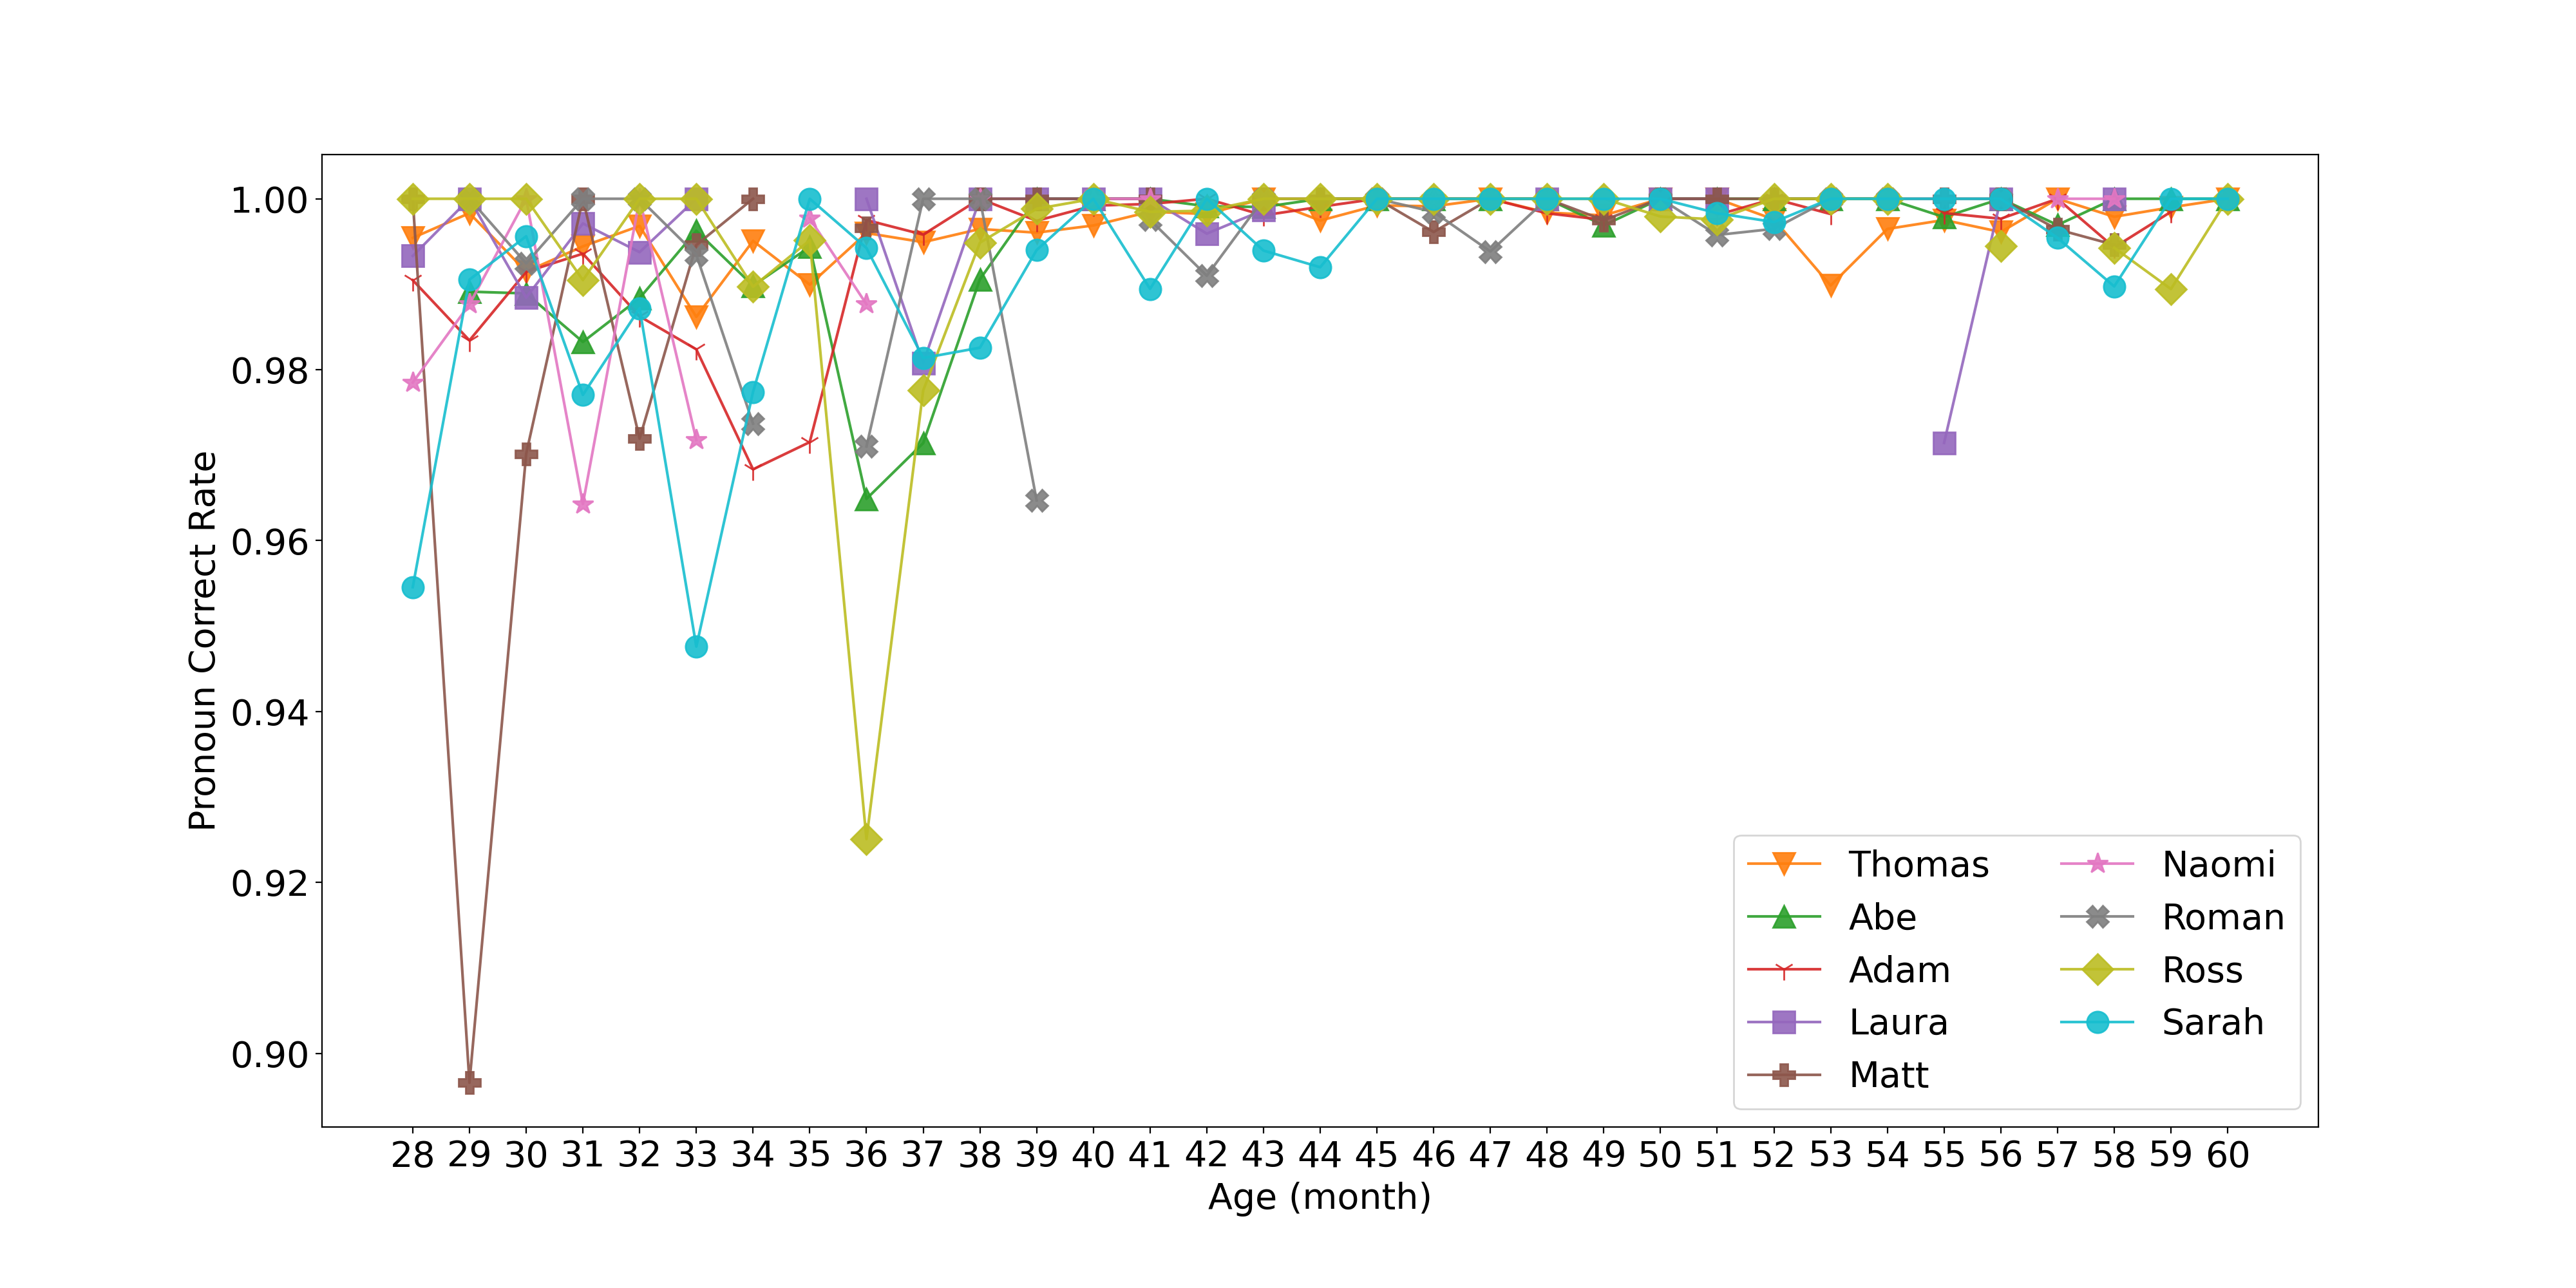
\includegraphics[scale = 0.35, width = \linewidth]{graph/Age1month.png}
\vspace{-2em}
\caption{Age and Pronoun Correct Rate per age point for with longitudinal data and cross-sectional data }
\label{fig:1}
\end{figure}
\FloatBarrier

The pronoun correct rate has a very noisy pattern at the early age points and stabilizes roughly after the age point of 3;4 (40 months). To get a more clear visualization for the early age points, the pronoun correct rate were averaged per 5 age points and the new plot is shown in Figure \ref{fig:2}.
\FloatBarrier
\begin{figure}[h]
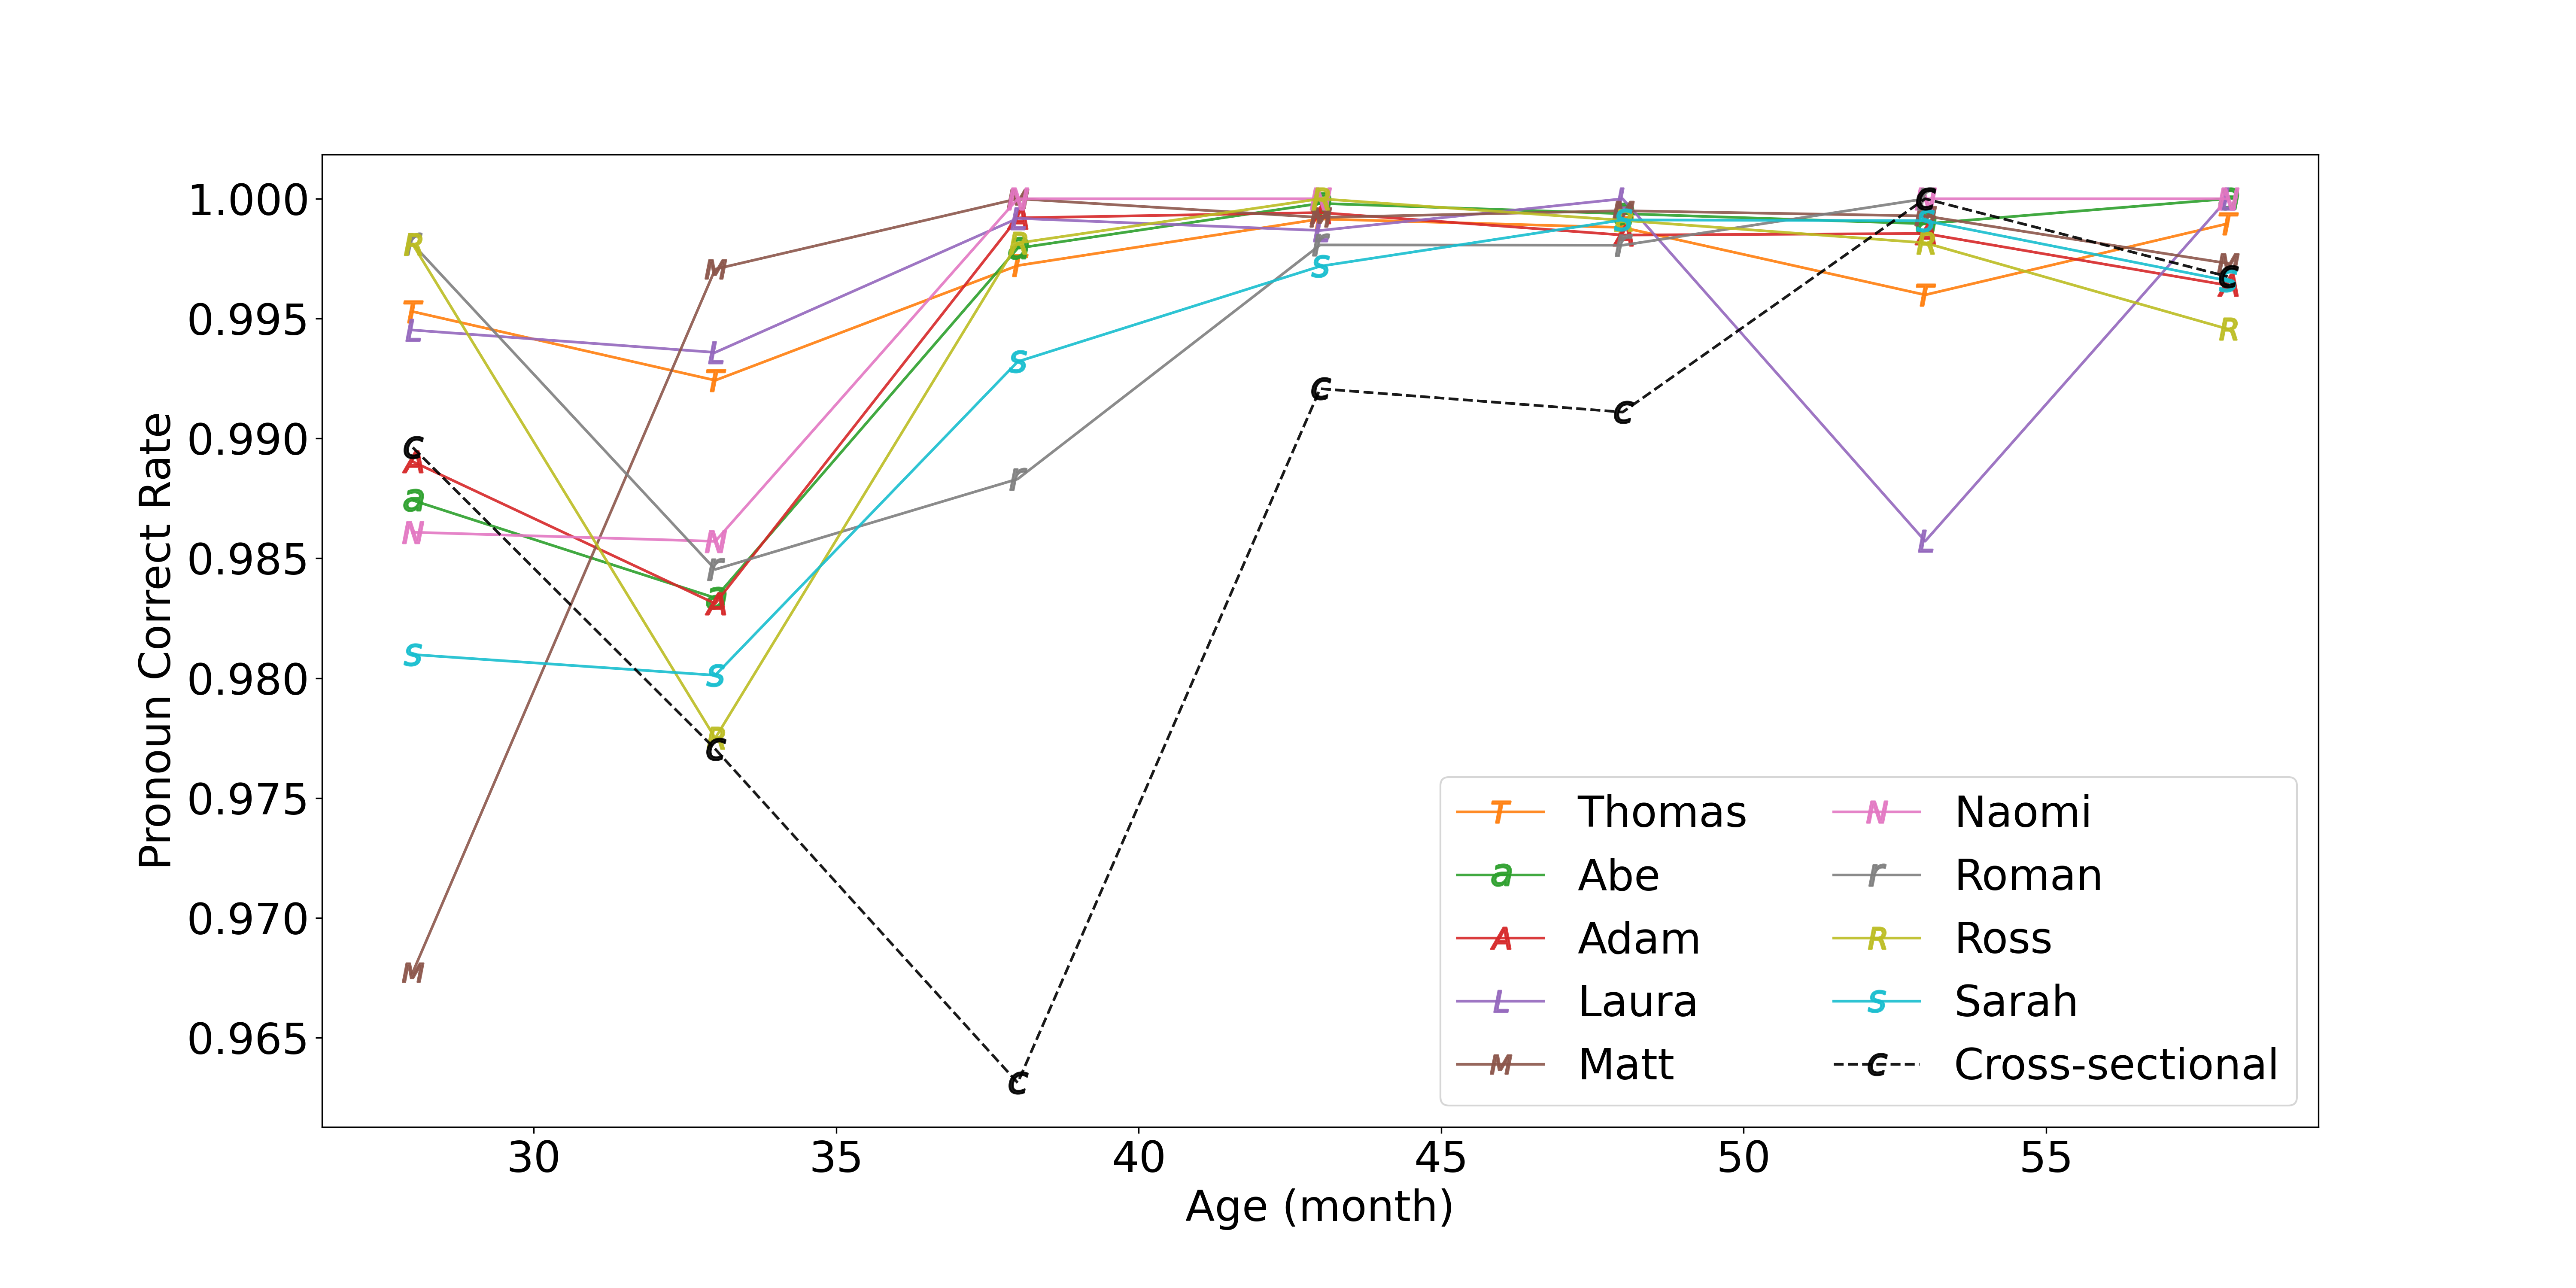
\includegraphics[scale = 0.35, width = \linewidth]{graph/Age5month.png}
\vspace{-2em}
\caption{Age and Pronoun Correct Rate per 5 age points}
\label{fig:2}
\end{figure}
\FloatBarrier
The colored solid lines represent each individual child's pronoun correct rate and the dashed black line represents the cross-sectional data. The longitudinal children's pronoun correct rate seems to resemble a U-shaped pattern, that most children start with a relatively high correct rate and then experience a dip at around age 2;9 (33 months) and return to high correct rate roughly after 3;7 (40 months). However, the position of the dip in longitudinal data is slightly different from the dip in the cross-sectional data: the pronoun correct rate dropped earlier for the children with longitudinal data than the children with cross-sectional data. It is unclear why the pronoun correct rate dropped at different age for longitudinal children and cross-sectional children. One possible explanation could be sampling error, since the cross-sectional data were averaged over 9 corpora collected at different times, ranging from 1977 - 2013. 

\FloatBarrier
\begin{table}[h]
\centering
\small
\caption{Summary of children's age range, mlu range, total pronouns, total input pronouns and total errors}
\label{table:2}
\begin{tabular}{llllllll}
\hline
\textbf{Name} & \textbf{{\begin{tabular}[c]{@{}l@{}}Total\\files \end{tabular}}}\footnote{Diary files were not included in this study. For example, Lara had 225 diary files that were not included in the study.} & \textbf{Age range} & \textbf{MLU range} & \textbf{\begin{tabular}[c]{@{}l@{}}Children's\\ Total\\ Pronoun\end{tabular}} & \textbf{\begin{tabular}[c]{@{}l@{}}Total\\Input\\ pronoun\end{tabular}} & \textbf{{\begin{tabular}[c]{@{}l@{}}Total\\Errors \end{tabular}}} & \textbf{\begin{tabular}[c]{@{}l@{}}Correct \\ Rate\end{tabular}} \\ \hline
Anne & 40 & 1;10 - 2;9 & 1.75 - 4.15 & 4957 & 18707 & 54 & 98.91\% \\
Aran & 53 & 1;11 - 2;11 & 1.46 - 5.02 & 10174 & 43339 & 24 & 99.76\% \\
Barbara & 14 & 2;4 - 4;2 & 3.37 - 6.47 & 1339 & 5052 & 7 & 99.48\% \\
Becky & 35 & 2;0 - 2;11 & 1.53 - 3.97 & 6893 & 14524 & 41 & 99.41\% \\
Carl & 33 & 1;9 - 2;8 & 2.22 - 4.36 & 5446 & 10398 & 32 & 99.41\% \\
Conor & 14 & 3;8 - 4;6 & 1.87 - 5.71 & 1993 & 8051 & 14 & 99.30\% \\
Courtney & 7 & 3;4 - 4;0 & 5.13 - 6.68 & 1398 & 1727 & 6 & 99.57\% \\
David & 14 & 2;0 - 4;2 & 2.32 - 6.41 & 1013 & 3219 & 3 & 99.70\% \\
Dominic & 36 & 1;11 - 2;11 & 1.34 - 4.08 & 4787 & 18519 & 47 & 99.02\% \\
Eleanor & 181 & 2;0 - 3;1 & 2.12 - 4.25 & 28834 & 59462 & 80 & 99.72\% \\
Fraser & 217 & 2;0 - 3;1 & 1.70 - 5.7 & 37480 & 92975 & 67 & 99.82\% \\
Gail & 35 & 2;0 - 2;11 & 1.87 - 4.33 & 4690 & 16029 & 63 & 98.66\% \\
Joel & 35 & 1;11 - 2;10 & 1.41 - 3.92 & 4936 & 15207 & 24 & 99.51\% \\
John & 32 & 1;11 - 2;11 & 1.92 - 3.78 & 2168 & 10276 & 8 & 99.63\% \\
Johnny & 7 & 3;6 - 4;4 & 3.93 - 4.52 & 861 & 507 & 4 & 99.54\% \\
Lara & 125 & 1;9 - 3;4 & 1.85 - 5.35 & 153054 & 40920 & 63 & 99.75\% \\
Liz & 34 & 1;11 - 2;11 & 1.52 - 4.79 & 5048 & 10708 & 31 & 99.39\% \\
Michelle & 14 & 2;5 - 4;5 & 3.0 - 6.87 & 2386 & 3979 & 31 & 98.70\% \\
Nicole & 34 & 2;1 - 3;0 & 1.26 - 3.61 & 2286 & 17860 & 51 & 97.77\% \\
Rachel & 9 & 2;6 - 3;2 & 2.8 - 6.33 & 663 & 2756 & 42 & 93.67\% \\
Ruth & 33 & 1;11 - 3;0 & 1.63 - 4.34 & 4077 & 19657 & 971 & 76.18\% \\
Stuart & 11 & 3;5 - 4;5 & 4.51 - 6.34 & 2352 & 2720 & 22 & 99.06\% \\
Thomas & 379 & 2;0 - 5;0 & 1.55 - 6.92 & 48115 & 226908 & 197 & 99.59\% \\
Warren & 36 & 1;10 - 2;10 & 2.02 - 4.71 & 4008 & 14818 & 96 & 97.60\% \\
Peter & 20 & 1;9 - 3;2 & 1.47 - 6.66 & 7637 & 2527 & 89 & 98.83\% \\
Laura & 200 & 1;5 - 7;0 & 1.0 - 6.69 & 9895 & 14280 & 82 & 99.17\% \\
Adam & 55 & 2;3 - 5;2 & 2.41 - 6.48 & 23726 & 13172 & 90 & 99.62\% \\
Eve & 20 & 1;6 - 2;3 & 2.1 - 4.99 & 4217 & 6458 & 39 & 99.08\% \\
Sarah & 139 & 2;3 - 5;1 & 1.59 - 7.77 & 15344 & 18512 & 110 & 99.28\% \\
Jimmy & 26 & 2;2 - 2;10 & 3.51 - 5.8 & 2702 & 3736 & 31 & 98.85\% \\
Shem & 47 & 2;3 - 3;2 & 4.32 - 12.03 & 9176 & 2207 & 19 & 99.79\% \\
Naomi & 93 & 1;3 - 4;9 & 1.3 - 7.79 & 5200 & 6466 & 60 & 98.85\% \\
Ross & 409 & 1;4 - 7;8 & 1.7 - 21.25 & 24560 & 41774 & 99 & 99.60\% \\
She & 10 & 1;8 - 2;5 & 2.23 - 3.54 & 706 & 2355 & 21 & 97.03\% \\
Tow & 10 & 1;7 - 2;5 & 1.86 - 5.08 & 946 & 3790 & 34 & 96.41\% \\
Nina & 52 & 2;0 - 3;4 & 2.26 - 6.17 & 11740 & 25694 & 501 & 95.73\% \\
Abe & 210 & 2;5 - 5;0 & 3.69 - 10.58 & 24547 & 18526 & 130 & 99.47\% \\
Trevor & 26 & 2;1 - 4;0 & 4.28 - 8.12 & 2819 & 5222 & 17 & 99.40\% \\
Ben & 11 & 2;4 - 3;4 & 4.97 - 6.88 & 1634 & 1177 & 50 & 96.94\% \\
Emily & 23 & 2;6 - 4;6 & 4.66 - 9.54 & 5067 & 144 & 15 & 99.70\% \\
Emma & 27 & 2;8 - 4;8 & 3.71 - 6.4 & 3458 & 2648 & 5 & 99.86\% \\
Jillian & 22 & 2;1 - 2;10 & 2.76 - 7.16 & 2669 & 2795 & 5 & 99.81\% \\
Matt & 57 & 2;3 - 5;0 & 2.89 - 11.29 & 6586 & 19759 & 34 & 99.48\% \\
Roman & 42 & 2;3 - 4;8 & 2.98 - 12.11 & 6047 & 4745 & 33 & 99.45\% \\
Nathaniel & 47 & 2;6 - 3;9 & 1.82 - 6.45 & 2193 & 10329 & 14 & 99.36\% \\
Geraldine & 10 & 1;6 - 2;5 & 1.35 - 5.43 & 598 & 1945 & 3 & 99.50\% \\ \hline
\end{tabular}
\end{table}
\FloatBarrier

\FloatBarrier
\begin{table}[]
\small
\centering
\caption{Spearman's Correlation between Pronoun Correct Rate and Age, MLU, Children's total words production, Children's pronoun production, Total Input Pronoun}
\begin{tabular}{ll|lllll}
\toprule
 & &\multicolumn{5}{c}{\textbf{Correlation (r) with Pronoun Correct Rate}} \\
\hline
\textbf{Child} & \textbf{{\begin{tabular}[c]{@{}l@{}}N (age points)\\(age range)\end{tabular}}}& \textbf{Age} & \textbf{MLU} & \textbf{\begin{tabular}[c]{@{}l@{}}Children's\\ Total Words\end{tabular}} & \textbf{\begin{tabular}[c]{@{}l@{}}Children's\\ Total Pronouns\end{tabular}} & \textbf{\begin{tabular}[c]{@{}l@{}}Total Input\\ Pronouns\end{tabular}}\\
\hline
Anne&11 (1;10 - 2;9)&-0.16&-0.04&-0.38&-0.33&-0.29\\
Aran&12 (1;11 - 2;11)&\textbf{0.77**}&\textbf{0.68*}&\textbf{0.79**}&\textbf{0.78**}&-0.05\\
Barbara&10 (2;4 - 4;2)&-0.14&0.3&-0.12&-0.08&-0.08\\
Becky&12 (2;0 - 2;11)&-0.36&-0.57&-0.31&-0.34&0.49\\
Carl&12 (1;9 - 2;8)&-0.07&0.22&0.19&-0.02&0.42\\
Conor&9 (3;8 - 4;6)&-0.34&\textbf{-0.94***}&-0.38&-0.42&-0.43\\
Courtney&5 (3;4 - 4;0)&0&0&-0.35&-0.35&0\\
David&12 (2;0 - 4;2)&-0.16&-0.23&-0.44&-0.38&0.19\\
Dominic&12 (1;11 - 2;11)&\textbf{-0.77**}&\textbf{-0.77**}&\textbf{-0.62*}&\textbf{-0.81**}&-0.46\\
Eleanor&14 (2;0 - 3;1)&0.45&0.42&0.5&0.52&\textbf{0.83***}\\
Fraser&14 (2;0 - 3;1)&\textbf{0.60*}&0.5&0.42&\textbf{0.57*}&\textbf{0.57*}\\
Gail&11 (2;0 - 2;11)&0.35&0.25&\textbf{-0.43}&-0.11&\textbf{0.51}\\
Joel&11 (1;11 - 2;10)&0.12&0.09&0.31&0.11&\textbf{0.75**}\\
John&12 (1;11 - 2;11)&0&-0.02&-0.35&-0.11&0.08\\
Johnny&5 (3;6 - 4;4)&-0.15&-0.67&-0.36&-0.67&-0.67\\
Lara&19 (1;9 - 3;4)&\textbf{0.61**}&\textbf{0.60**}&0.3&\textbf{0.55*}&0.33\\
Liz&12 (1;11 - 2;11)&0.46&0.39&-0.12&0.15&-0.35\\
Michelle&9 (2;5 - 4;5)&-0.39&-0.14&-0.31&-0.31&0.29\\
Nicole&11 (2;1 - 3;0)&\textbf{-0.85***}&\textbf{-0.85***}&\textbf{-0.76***}&\textbf{-0.82***}&-0.11\\
Rachel&5 (2;6 - 3;2)&0.72&0.87&-0.87&-0.36&0.1\\
Ruth&13 (1;11 - 3;0)&0.4&0.45&0.36&0.33&0.51\\
Stuart&7 (3;5 - 4;5)&\textbf{0.83*}&0.09&-0.25&-0.11&-0.04\\
Thomas&36 (2;0 - 5;0)&\textbf{0.51**}&\textbf{0.58**}&\textbf{0.39*}&\textbf{0.39*}&0.1\\
Warren&12 (1;10 - 2;10)&0.05&-0.03&0.09&0.24&0.29\\
Peter&14 (1;9 - 3;2)&0.11&0.15&0.07&0.09&-0.37\\
Laura&34 (1;5 - 7;0)&\textbf{0.60***}&\textbf{0.48**}&\textbf{0.57***}&\textbf{0.50**}&\textbf{0.40*}\\
Adam&31 (2;3 - 5;2)&\textbf{0.61***}&\textbf{0.62***}&\textbf{0.50**}&\textbf{0.45*}&0.11\\
Eve&10 (1;6 - 2;3)&\textbf{-0.74*}&\textbf{-0.69*}&\textbf{-0.66*}&\textbf{-0.67*}&-0.02\\
Sarah&35 (2;3 - 5;1)&\textbf{0.63***}&\textbf{0.60***}&\textbf{0.46**}&0.28&0.04\\
Jimmy&6 (2;2 - 2;10)&-0.6&-0.6&0.31&-0.09&0.31\\
Shem&12 (2;3 - 3;2)&0.04&-0.03&0.04&0.25&0.39\\
Naomi&23 (1;3 - 4;9)&\textbf{0.42*}&\textbf{0.43*}&0.25&0.33&0.18\\
Ross&62 (1;4 - 7;8)&0.14&-0.07&-0.17&-0.19&0.09\\
She&9 (1;8 - 2;5)&\textbf{0.78*}&0.57&0.45&\textbf{0.72*}&0.52\\
Tow&9 (1;7 - 2;5)&0.31&0.29&0&0&-0.15\\
Nina&15 (2;0 - 3;4)&\textbf{0.83***}&\textbf{0.86***}&\textbf{0.62*}&\textbf{0.68**}&0.26\\
Abe&32 (2;5 - 5;0)&\textbf{0.69***}&\textbf{0.38*}&-0.26&-0.24&\textbf{-0.46**}\\
Trevor&10 (2;1 - 4;0)&0.01&-0.49&-0.07&-0.05&0.25\\
Ben&8 (2;4 - 3;4)&0.36&0.4&-0.19&0.5&\textbf{0.71*}\\
Emily&13 (2;6 - 4;6)&0.07&-0.18&-0.4&-0.37&-0.25\\
Emma&16 (2;8 - 4;8)&0.47&0.41&0.44&0.43&-0.21\\
Jillian&7 (2;1 - 2;10)&-0.08&-0.16&-0.45&-0.35&0.37\\
Matt&29 (2;3 - 5;0)&0.27&0.28&0.29&0.11&0.09\\
Roman&24 (2;3 - 4;8)&0.15&-0.06&-0.19&-0.07&0.17\\
Nathaniel&10 (2;6 - 3;9)&0.35&\textbf{0.63*}&0.12&0.52&0.22\\
Geraldine&7 (1;6 - 2;5)&0.4&0.4&-0.04&0.09&0.04\\
\bottomrule
\end{tabular}
\end{table}
\FloatBarrier


\FloatBarrier
\begin{table}[h]
\small
\centering
\caption{Pronoun Correct Rate at each age points for 9 children}
\label{table:4}
\begin{tabular}{c|lllllllll}
\hline
\textbf{{\begin{tabular}[c]{@{}c@{}}Age\\(month)\end{tabular}}} & \textbf{Thomas} & \textbf{Abe} & \textbf{Adam} & \textbf{Laura} & \textbf{Matt} & \textbf{Naomi} & \textbf{Roman} & \textbf{Ross} & \textbf{Sarah} \\ 
\toprule
28 & 99.54\% & N/A & 99.05\% & 99.33\% & 100.00\% & 97.85\% & N/A & 100.00\% & 95.45\% \\
29 & 99.83\% & 98.91\% & 98.34\% & 100.00\% & 89.66\% & 98.77\% & 100.00\% & 100.00\% & 99.05\% \\
30 & 99.15\% & 98.89\% & 99.15\% & 98.84\% & 97.01\% & 100.00\% & 99.24\% & 100.00\% & 99.56\% \\
31 & 99.44\% & 98.32\% & 99.36\% & 99.71\% & 100.00\% & 96.43\% & 100.00\% & 99.05\% & 97.70\% \\
32 & 99.68\% & 98.84\% & 98.62\% & 99.38\% & 97.19\% & 100.00\% & 100.00\% & 100.00\% & 98.72\% \\
33 & 98.62\% & 99.62\% & 98.24\% & 100.00\% & 99.46\% & 97.18\% & 99.34\% & 100.00\% & 94.76\% \\
34 & 99.51\% & 98.98\% & 96.83\% & N/A & 100.00\% & N/A & 97.37\% & 98.97\% & 97.74\% \\
35 & 99.00\% & 99.44\% & 97.15\% & N/A & N/A & 99.77\% & N/A & 99.51\% & 100.00\% \\
36 & 99.60\% & 96.49\% & 99.75\% & 100.00\% & 99.66\% & 98.77\% & 97.10\% & 92.51\% & 99.42\% \\
37 & 99.49\% & 97.14\% & 99.58\% & 98.08\% & N/A & N/A & 100.00\% & 97.76\% & 98.14\% \\
38 & 99.65\% & 99.06\% & 100.00\% & 100.00\% & 100.00\% & 100.00\% & 100.00\% & 99.49\% & 98.26\% \\
39 & 99.60\% & 100.00\% & 99.74\% & 100.00\% & 100.00\% & N/A & 96.47\% & 99.88\% & 99.40\% \\
40 & 99.69\% & 100.00\% & 99.92\% & 100.00\% & 100.00\% & 100.00\% & N/A & 100.00\% & 100.00\% \\
41 & 99.85\% & 100.00\% & 99.94\% & 100.00\% & 100.00\% & 100.00\% & 99.75\% & 99.85\% & 98.95\% \\
42 & 99.82\% & 99.91\% & 100.00\% & 99.59\% & N/A & N/A & 99.10\% & 99.86\% & 100.00\% \\
43 & 100.00\% & 99.90\% & 99.81\% & 99.87\% & 100.00\% & N/A & 100.00\% & 100.00\% & 99.39\% \\
44 & 99.74\% & 100.00\% & 99.91\% & N/A & 100.00\% & N/A & N/A & 100.00\% & 99.20\% \\
45 & 99.92\% & 100.00\% & 100.00\% & N/A & 100.00\% & N/A & 100.00\% & 100.00\% & 100.00\% \\
46 & 99.91\% & 100.00\% & 100.00\% & N/A & 99.61\% & 100.00\% & 99.85\% & 100.00\% & 100.00\% \\
47 & 100.00\% & 100.00\% & 100.00\% & N/A & 100.00\% & N/A & 99.38\% & 100.00\% & 100.00\% \\
48 & 99.84\% & 100.00\% & 99.83\% & 100.00\% & 100.00\% & N/A & 100.00\% & 100.00\% & 100.00\% \\
49 & 99.81\% & 99.69\% & 99.75\% & N/A & 99.75\% & N/A & N/A & 100.00\% & 100.00\% \\
50 & 100.00\% & 100.00\% & N/A & 100.00\% & 100.00\% & N/A & 100.00\% & 99.79\% & 100.00\% \\
51 & 100.00\% & 100.00\% & 99.81\% & 100.00\% & 100.00\% & N/A & 99.58\% & 99.76\% & 99.83\% \\
52 & 99.76\% & 100.00\% & 100.00\% & N/A & 100.00\% & N/A & 99.65\% & 100.00\% & 99.73\% \\
53 & 98.99\% & 100.00\% & 99.82\% & N/A & 100.00\% & N/A & 100.00\% & 100.00\% & 100.00\% \\
54 & 99.65\% & 100.00\% & N/A & N/A & 100.00\% & N/A & 100.00\% & 100.00\% & 100.00\% \\
55 & 99.75\% & 99.79\% & 99.83\% & 97.14\% & 100.00\% & N/A & N/A & N/A & 100.00\% \\
56 & 99.61\% & 100.00\% & 99.77\% & 100.00\% & 100.00\% & N/A & 100.00\% & 99.45\% & 100.00\% \\
57 & 100.00\% & 99.69\% & 100.00\% & N/A & 99.64\% & 100.00\% & N/A & N/A & 99.54\% \\
58 & 99.79\% & 100.00\% & 99.43\% & 100.00\% & 99.46\% & 100.00\% & N/A & 99.43\% & 98.97\% \\
59 & 99.90\% & 100.00\% & 99.85\% & N/A & N/A & N/A & N/A & 98.94\% & 100.00\% \\
60 & 100.00\% & 100.00\% & N/A & N/A & 100.00\% & N/A & N/A & 100.00\% & 100.00\% \\ 
\bottomrule
\end{tabular}
\end{table}
\FloatBarrier

\subsubsection{Does Pronoun Case Error Display U-shaped Pattern?}
The U-shaped developmental trajectory has been observed in a wide variety of learning contexts \citep[for a review, see][]{siegler2004u}. It is especially interesting in language development since it contradicts the idea that language acquisition is monotonic. If the pronoun case errors display a U-shaped pattern, explanations for such errors should account for the non-monotonic developmental pattern too, which provides an important criteria to evaluate the effectiveness of different explanations. 

It's difficult to judge whether the pronoun case errors follow a U-shaped pattern. One challenge is that there is no accurate definition of the U-shaped developmental curve. The U-shaped pattern has been loosely described as a three-step process: good performance followed by bad performance followed by good performance again. However, it's difficult to decide what is good performance and what is bad performance in the pronoun case error context where most of the children have an extremely low error rate. In Figure \ref{fig:2}, the plot between age and pronoun correct rate does display the shape of `U', but the difference between the nadir (96.5\%) and the zenith (100\%) is so small that it is unclear whether there is meaningful improvement.

Most studies reporting a U-shaped developmental pattern did not plot the detailed correct rate with age to prove that there is a U-shaped pattern. Instead, they showed that the performance at a later age is significantly worse than an earlier age, but eventually get better. For example, \cite{namy2004changing} reported that both 18-month group and 4-year-old group had better performance on mapping arbitary gestures than 26-month old group. In order to test if pronoun correct rate at a certain age is  worse the other ages, all the months in cross-sectional data were divided into 7 groups with 5 months apart to ensure that each group have enough samples. Table \ref{table:KW} shows the mean and median pronoun correct rate for 7 different age groups. A Kruskal-Wallis test shows that there is no significant difference in pronoun correct rate among age groups, H(6) = 8.57, p = 0.20. This result suggests that even there is a dip of pronoun correct rate at around 2;9 - 3;2, the change is not significant. Based on the cross-sectional data, it's difficult to conclude if there is a U-shaped pattern. 
\FloatBarrier
\begin{table}[h]
\centering
\caption{Mean and Median Pronoun Correct Rate for 7 age groups }
\label{table:KW}
\begin{tabular}{llll}
\toprule
\begin{tabular}[c]{@{}c@{}}Age Group \\(month)\end{tabular} & N & Mean & Median \\
\hline
\textless{}26 & 18 & 98.83\% & 100\% \\
26 - 30 & 35 & 99.06\% & 100\%\\
31 - 35 & 29 & 98.97\% & 100\%\\
36 - 40 & 18 & 96.01\% & 100\% \\
41 - 45 & 32 & 99.65\% & 100\% \\
46 - 50 & 65 & 99.06\% & 100\% \\
\textgreater{}50 & 14 & 98.71\% & 100\%\\
\bottomrule
\end{tabular}
\end{table}
\FloatBarrier

For longitudinal data, since there are not enough samples for different age groups,  Kruskal-Wallis test can not be used to test if the pronoun correct rate is significantly different at different ages. Instead, the longitudinal change in the pronoun correct rate were compared to the correct rate on past-tense verbs. \cite{marcus1992overregularization}'s study on past-tense verb overregularization errors reported a U-shaped development pattern with detailed correct rate over 4 children's (Adam, Eve, Sarah, Abe) longitudinal data. To compare the shape and change of correct rate, Adam's, Sarah's and Abe's past-tense verb correct rate and pronoun correct rate were plotted together in Figure \ref{fig:3}. The pronoun correct rate stabilized above 95\% for all ages, while verb correct rate is more has more variations at different age points. Again, the comparison with past-tense verb correct rate shows that the changes in pronoun correct rate are too trivial to be meaningful.  

In sum, the plot between age and pronoun correct rate displays the shape of `U' in both longitudinal and cross-sectional data. However, the pronoun correct rate at different ages are all very close to 100\%, making the change in the correct rate not so meaningful. Therefore, no conclusion about U-shaped developmental pattern can be drawn. 
 

\FloatBarrier
\begin{figure}[h]
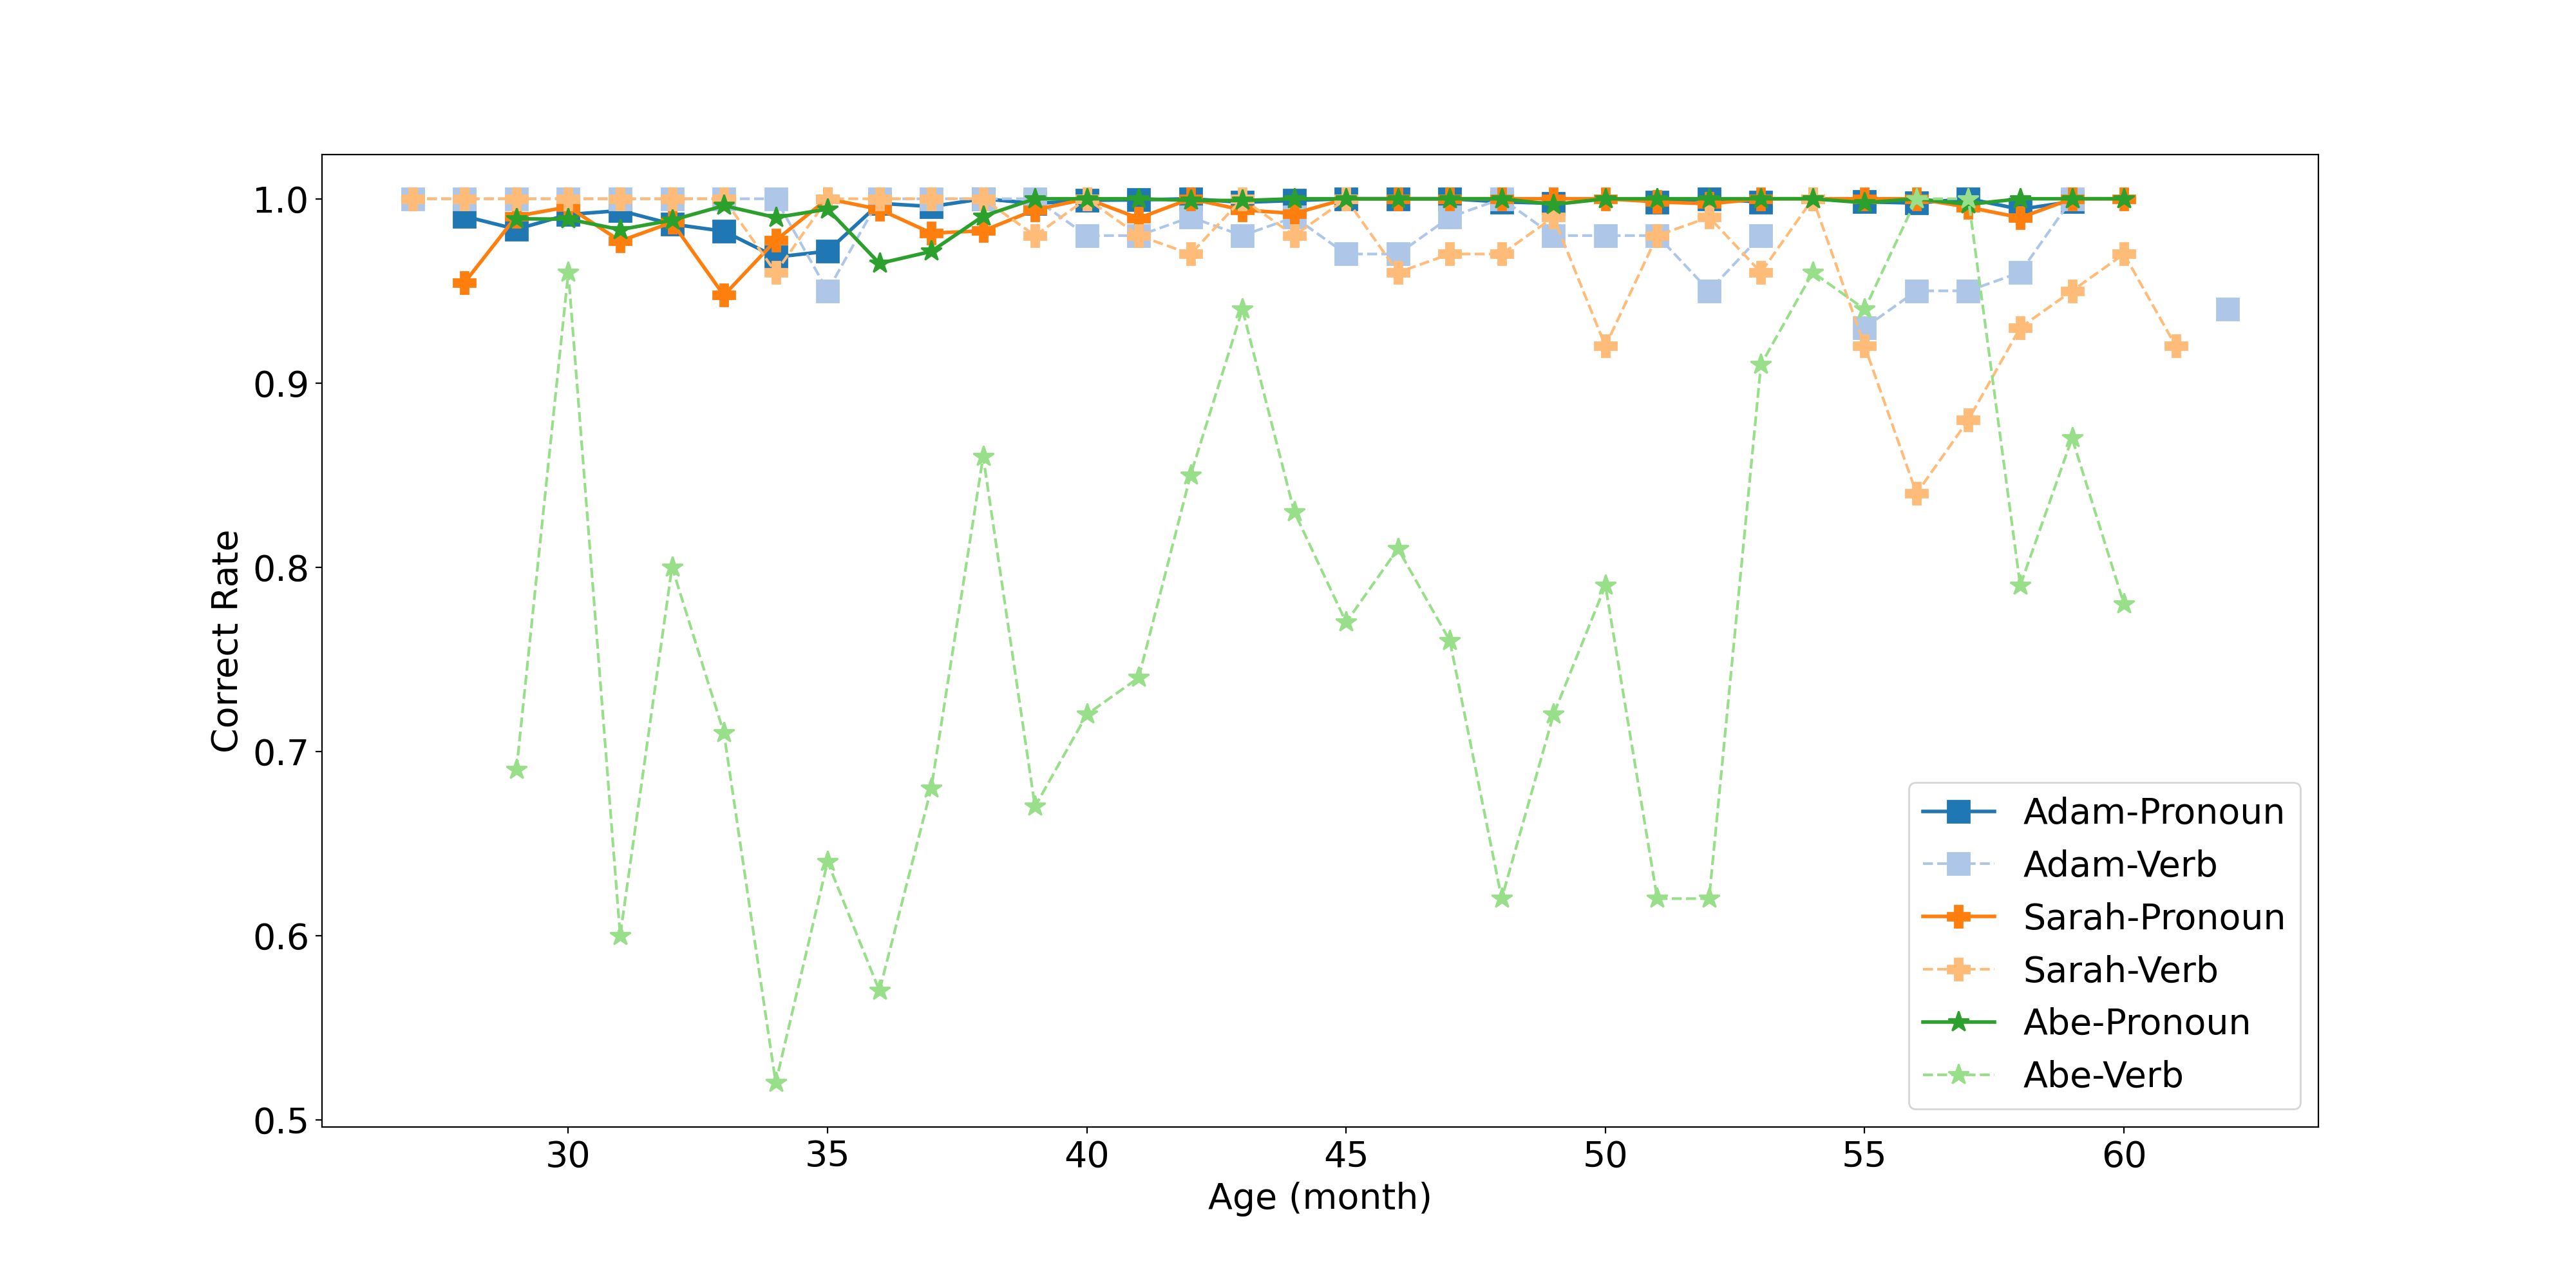
\includegraphics[scale = 0.35, width = \linewidth]{graph/AgeVerb.png}
\vspace{-3em}
\caption{Pronoun Correct Rate VS Verb Correct Rate for Adam, Abe and Sarah}
\label{fig:3}
\end{figure}
\FloatBarrier



\subsubsection{Different types of Pronoun Case Errors}
Children make many types of pronoun case errors as shown in previous sections. This subsection investigates the frequency of different types of pronoun case errors. The summary of pronoun case error data is shown in Table \ref{table:errordata}. 244,874 total pronouns were found produced by children with longitudinal recordings. \textit{`I'},\textit{`my'} and \textit{`me'} are the most frequently used pronouns by the children; and \textit{`us'}, \textit{`their'} and \textit{`our'} are the least used pronouns. There were 3421 errors, with an average error rate of 1.39\%. There were five types of errors: nominative case used as an object (NOM for OBJ), objective case used as a subject (OBJ for NOM) or a determiner (OBJ for GEN), genitive case used as a subject (GEN for NOM) or an object (GEN for OBJ). The most common errors occurred on pronoun \textit{`me'}, with 1579 \textit{`me'} used as \textit{`I'} and 165 \textit{`me'} used as \textit{`my'}. Seven pronouns (\textit{`I', `we', `she', `they', `his', `our'} and \textit{`their'}) have less than 10 errors. In addition, \textit{`I'} is the mostly substituted pronoun, with 1579 \textit{`I's} being substituted by \textit{`me'} and 485 \textit{`I's} being substituted by \textit{`my'}, as shown in Column `Subs' in Table \ref{table:errordata}. `Pronoun Correct Rate by Use' in Columb 6 is calculated as $1 - \displaystyle\frac{\text{Errors}}{\text{Total Tokens}}$.  For example, the correct rate by use for pronoun `I' is 1 -  $\displaystyle\frac{9}{118607} = 0.9999$. Most of the pronouns were used correctly over 95\% of the time, except for ‘me’ (91.80\%) and ‘her’ (91.14\%). `Pronoun Correct Rate by Argument Position' in Column 7 is calculated as the total argument positions (e.g. subject position, object position and determiner position) divided by the total positions that were  filled with a correct pronoun: $\displaystyle\frac{\text{Positions with correct pronoun}}{\text{Total argument positions}}$.  For example, for the subject position that requires a first person singular pronoun, the correct pronoun `\textit{I}' filled 118598 subject position, incorrect pronoun `\textit{me}' and `\textit{my}' filled 1579 and 485 subject positions respectively. Therefore, the correct rate by position for \textit{I} = $\displaystyle\frac{118607 - 9}{118607 - 9 + 1579 + 485} = 0.9829$. Most of the argument positions were filled with the correct pronoun over 98\% of the time, except for two positions: ‘she’ only filled 92.32\% of subject positions that required a third-person singular feminine pronoun and ‘their’ only filled 89.70\% of determiner positions that required a third-person plural pronoun. 

In addition, different types of errors are not equally popular among children. Children's errors are concentrated on three types of OBJ for NOM errors: 41 children made `me-for-I' error; 36 children made `them-for-they' error and 30 children made `her-for-she' error. Four types of errors (`she-for-her', `we-for-us', `they-for-them' and `our-for-we') had less than 5 children that made errors. Children don't make the same amount of errors on different error types. For some error types, children usually make that error once or twice. For example for `she-for-her' error, the maximum error per child is 1 and there were 4 children who made such error, meaning that each child only made `she-for-her' error once. For other types of errors, there might be one or two children's errors accounted for a majority of the error tokens. For example, of total 1579 `me-for-I' errors, 858 errors were made by one child. 
 
\FloatBarrier
\begin{table}[h]
\footnotesize
\caption{Summary of Pronoun Case Error Data}
\label{table:errordata}
\begin{tabular}{c|cccccccc}
\hline
Pronoun & Tokens & Error Type & Errors & Subs & \begin{tabular}[c]{@{}l@{}}Pronoun\\ Correct\\ Rate by \\ Use\textsuperscript{a}\end{tabular} & \begin{tabular}[c]{@{}l@{}}Pronoun \\ Correct\\ Rate by\\ Argument\\ Position\textsuperscript{b}\end{tabular} & \begin{tabular}[c]{@{}l@{}}N children\\ made error\end{tabular} & \begin{tabular}[c]{@{}l@{}}Maximum\\ error/child\end{tabular} \\ \hline
I & 118607 & I-for-me & 9 & 2064 & 99.99\% & 98.29\% & 6 & 3 \\
he & 16966 & he-for-him & 27 & 157 & 99.84\% & 99.08\% & 14 & 8 \\
she & 4955 & she-for-her & 4 & 412 & 99.92\% & 92.32\% & 4 & 1 \\
we & 13525 & we-for-us & 4 & 14 & 99.97\% & 99.90\% & 3 & 2 \\
they & 9703 & they-for-them & 4 & 202 & 99.96\% & 97.96\% & 4 & 1 \\
me & 21280 & me-for-I & 1579 & 40 & \multirow{2}{*}{91.80\%} & \multirow{2}{*}{99.81\%} & 41 & 858 \\
 &  & me-for-my & 165 &  &  &  & 21 & 81 \\
him & 4732 & him-for-he & 148 & 27 & \multirow{2}{*}{95.79\%} & \multirow{2}{*}{99.24\%} & 26 & 26 \\
 &  & him-for-his & 51 &  &  &  & 11 & 30 \\
her & 4650 & her-for-she & 412 & 4 & 91.14\% & 99.94\% & 30 & 169 \\
us & 727 & us-for-we & 13 & 4 & 98.21\% & 99.73\% & 9 & 3 \\
them & 7181 & them-for-they & 194 & 4 & \multirow{2}{*}{95.95\%} & \multirow{2}{*}{99.94\%} & 36 & 42 \\
 &  & them-for-their & 97 &  &  &  & 23 & 17 \\
my & 35329 & my-for-I & 485 & 165 & \multirow{2}{*}{98.54\%} & 99.54\% & 25 & 124 \\
 &  & my-for-me & 31 &  &  &  & 7 & 8 \\
his & 5109 & his-for-he & 9 & 51 & 99.82\% & 99.01\% & 9 & 1 \\
our & 1265 & our-for-we & 1 & 0 & 99.92\% & 100.00\% & 1 & 1 \\
their & 845 & their-for-they & 8 & 97 & 99.05\% & 89.70\% & 6 & 2\\
\hline
\end{tabular}
\end{table}
\FloatBarrier

Why children's pronoun case errors  are concentrated on few types of errors such as `\textit{me}-for-\textit{I}' and `\textit{her}-for-\textit{she}'? One possible explanation is that the error rate is related to how often children use a certain pronoun or how often children hear a certain pronoun in the parents' input. A Spearman's test shows that for each pronoun, there is a strong positive correlation between children's pronoun production and parents' pronoun input ($r_s$ = 0.80**, p <0.001), but there is no significant correlation between pronoun correct rate by use and children's pronoun production ($r_s$ = 0.22, p = 0.45) or parents' pronoun input ($r_s$ = 0.43, p = 0.13). Similarly, pronoun correct rate by position is not correlated with children's pronoun production ($r_s$ = -0.09, p = 0.77), or with parents' pronoun input ($r_s$ = -0.07, p = 0.81). Figure \ref{fig:corrct} visualizes that pronoun correct rate by rate and by position are not proportional to children's pronoun production or parents' input. In addition, each pronoun's error tokens are not correlated with children's pronoun production ($r_s$ = 0.30, p = 0.30) or with parents' pronoun input ($r_s$ = -0.01, p = 0.96). The results indicate that children do not produce more errors on a pronoun simply because they use that pronoun or hear that pronoun more often. Instead, children's pronoun production could be related to pronoun case errors in another way: the more often children use a pronoun, the more likely that pronoun is to be substituted. For example, \textit{`I'} is the most used pronoun by children. There were only 9 \textit{`I'}-for-\textit{'me'} errors, whereas 2064 \textit{`I'}s were substituted with \textit{`me'} and \textit{'my'}. A Spearman's test shows that children's pronoun production is positively correlated with pronouns' substituted tokens ($r_s$ = 0.56*, p = 0.03). The substituted tokens are not correlated with parents' pronoun input ($r_s$ = 0.47, p = 0.09). Figure \ref{fig:errortoken} shows that the error tokens are not correlated with children's and parents' pronoun tokens, and substituted tokens are correlated with children's pronoun production.


\FloatBarrier
\begin{figure}[!h]
    \centering
    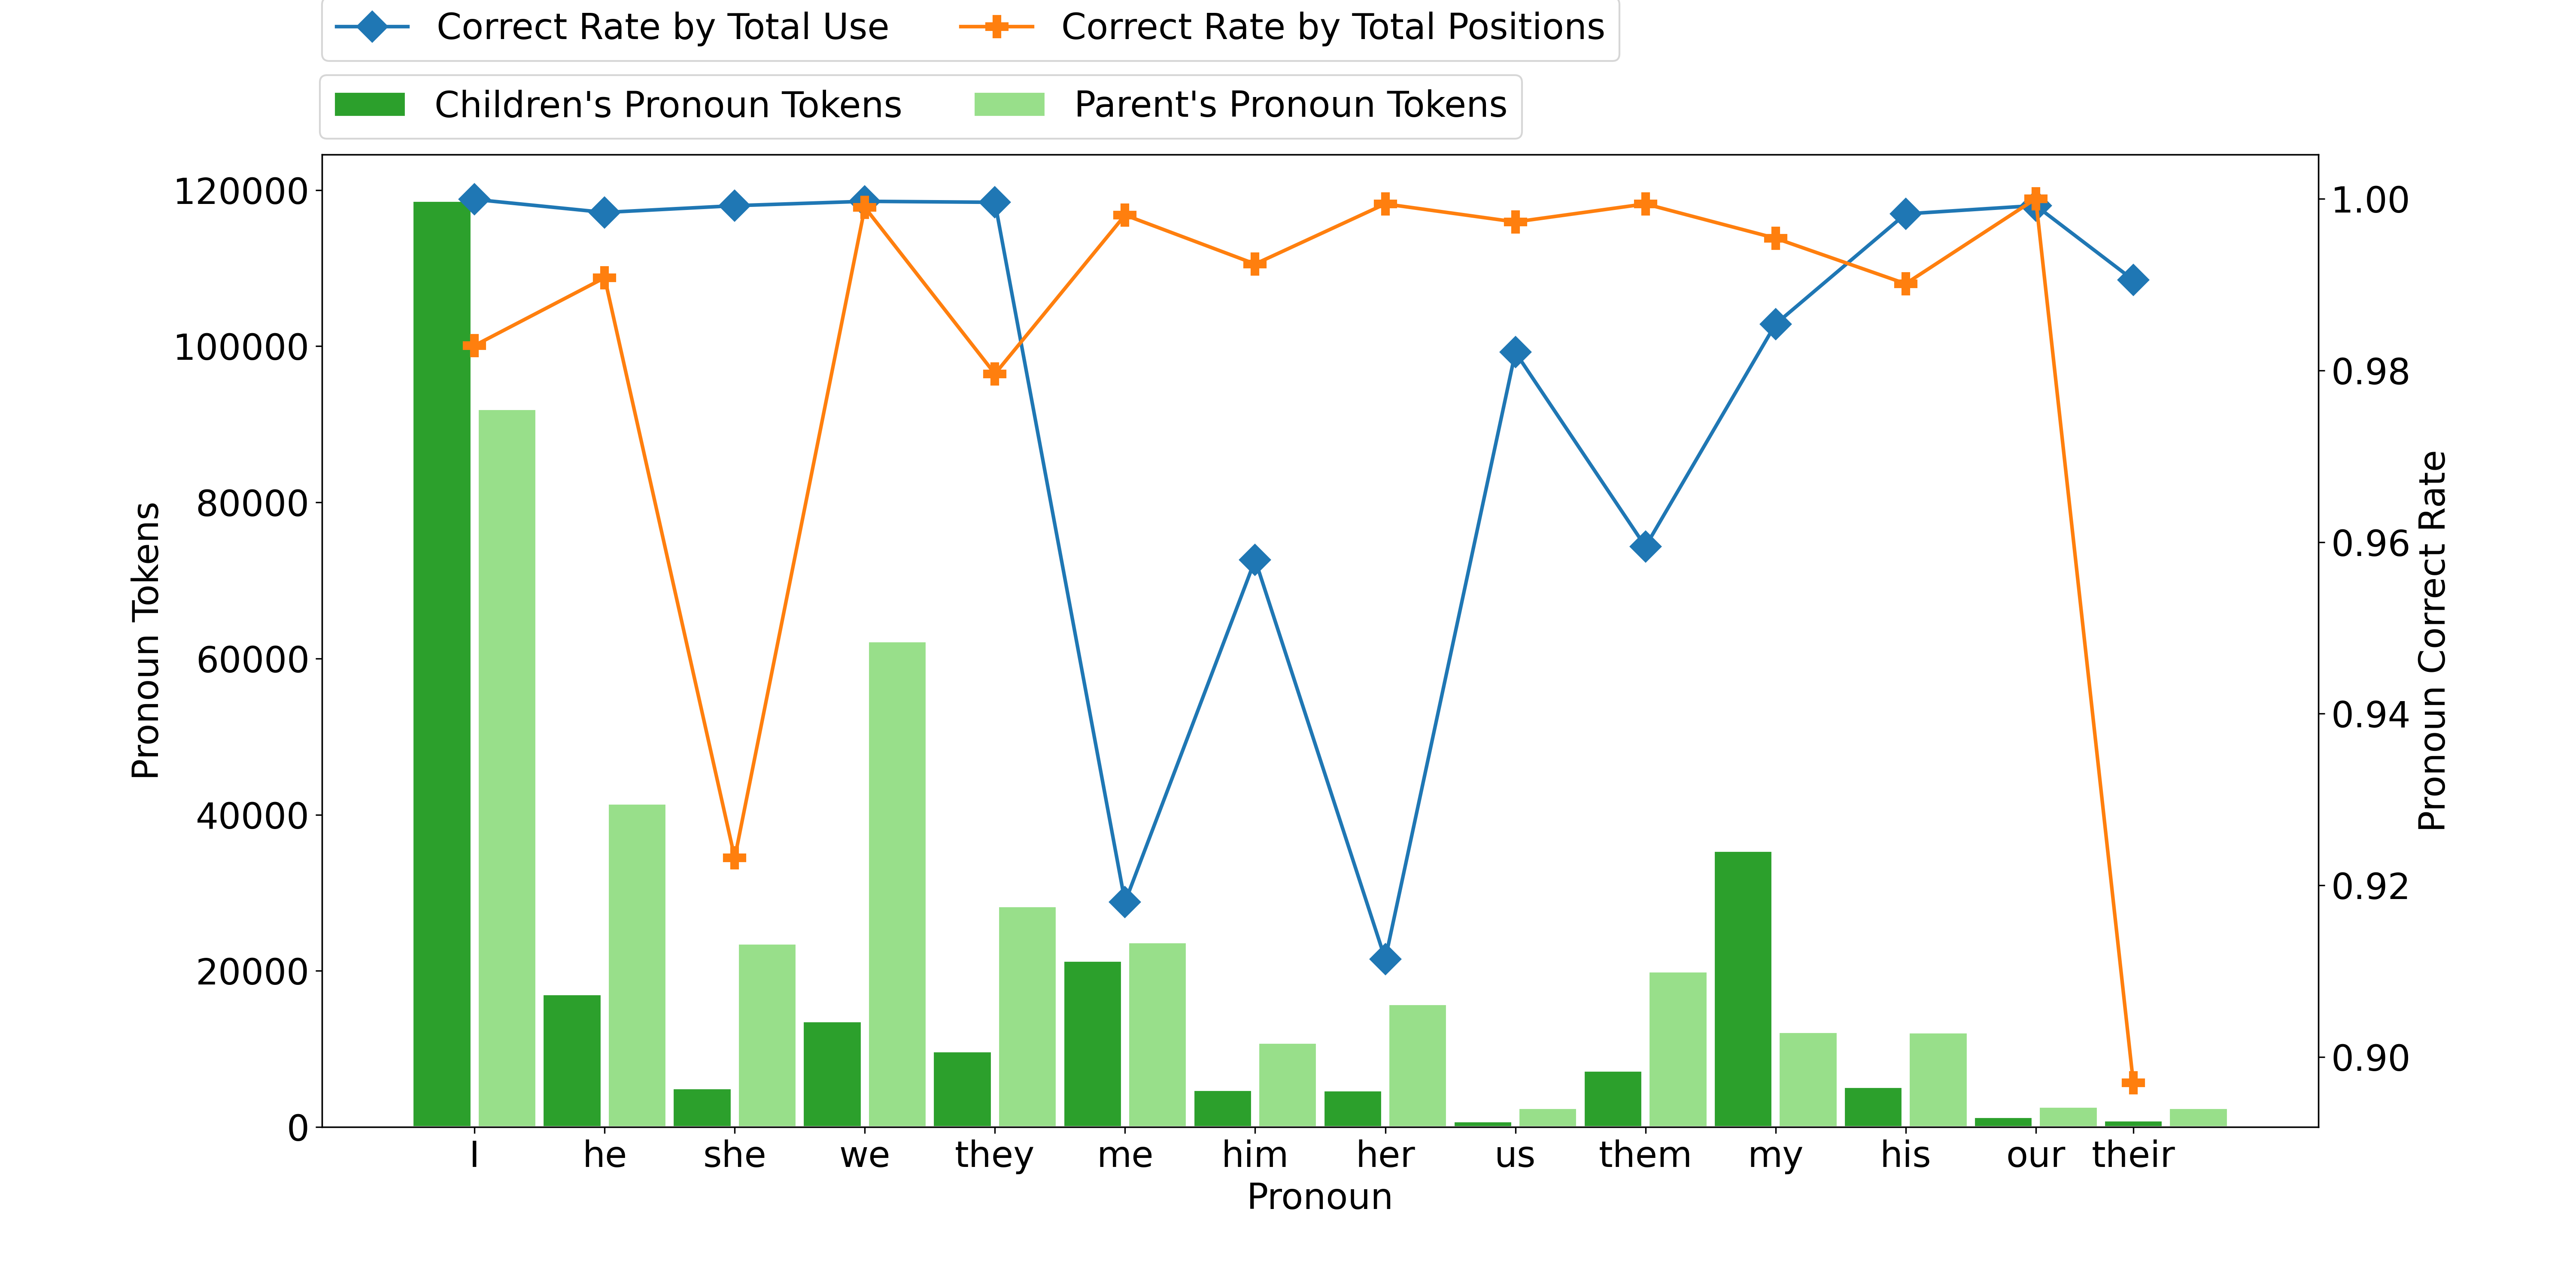
\includegraphics[scale = 0.35]{graph/PronounandRate.png}
    \vspace{-2em}
    \caption{Pronoun Correct Rate by Use and by Token and Pronoun Tokens by Parents and Children }
    \label{fig:corrct}
\end{figure}
\FloatBarrier
\FloatBarrier
\begin{figure}[!h]
    \centering
    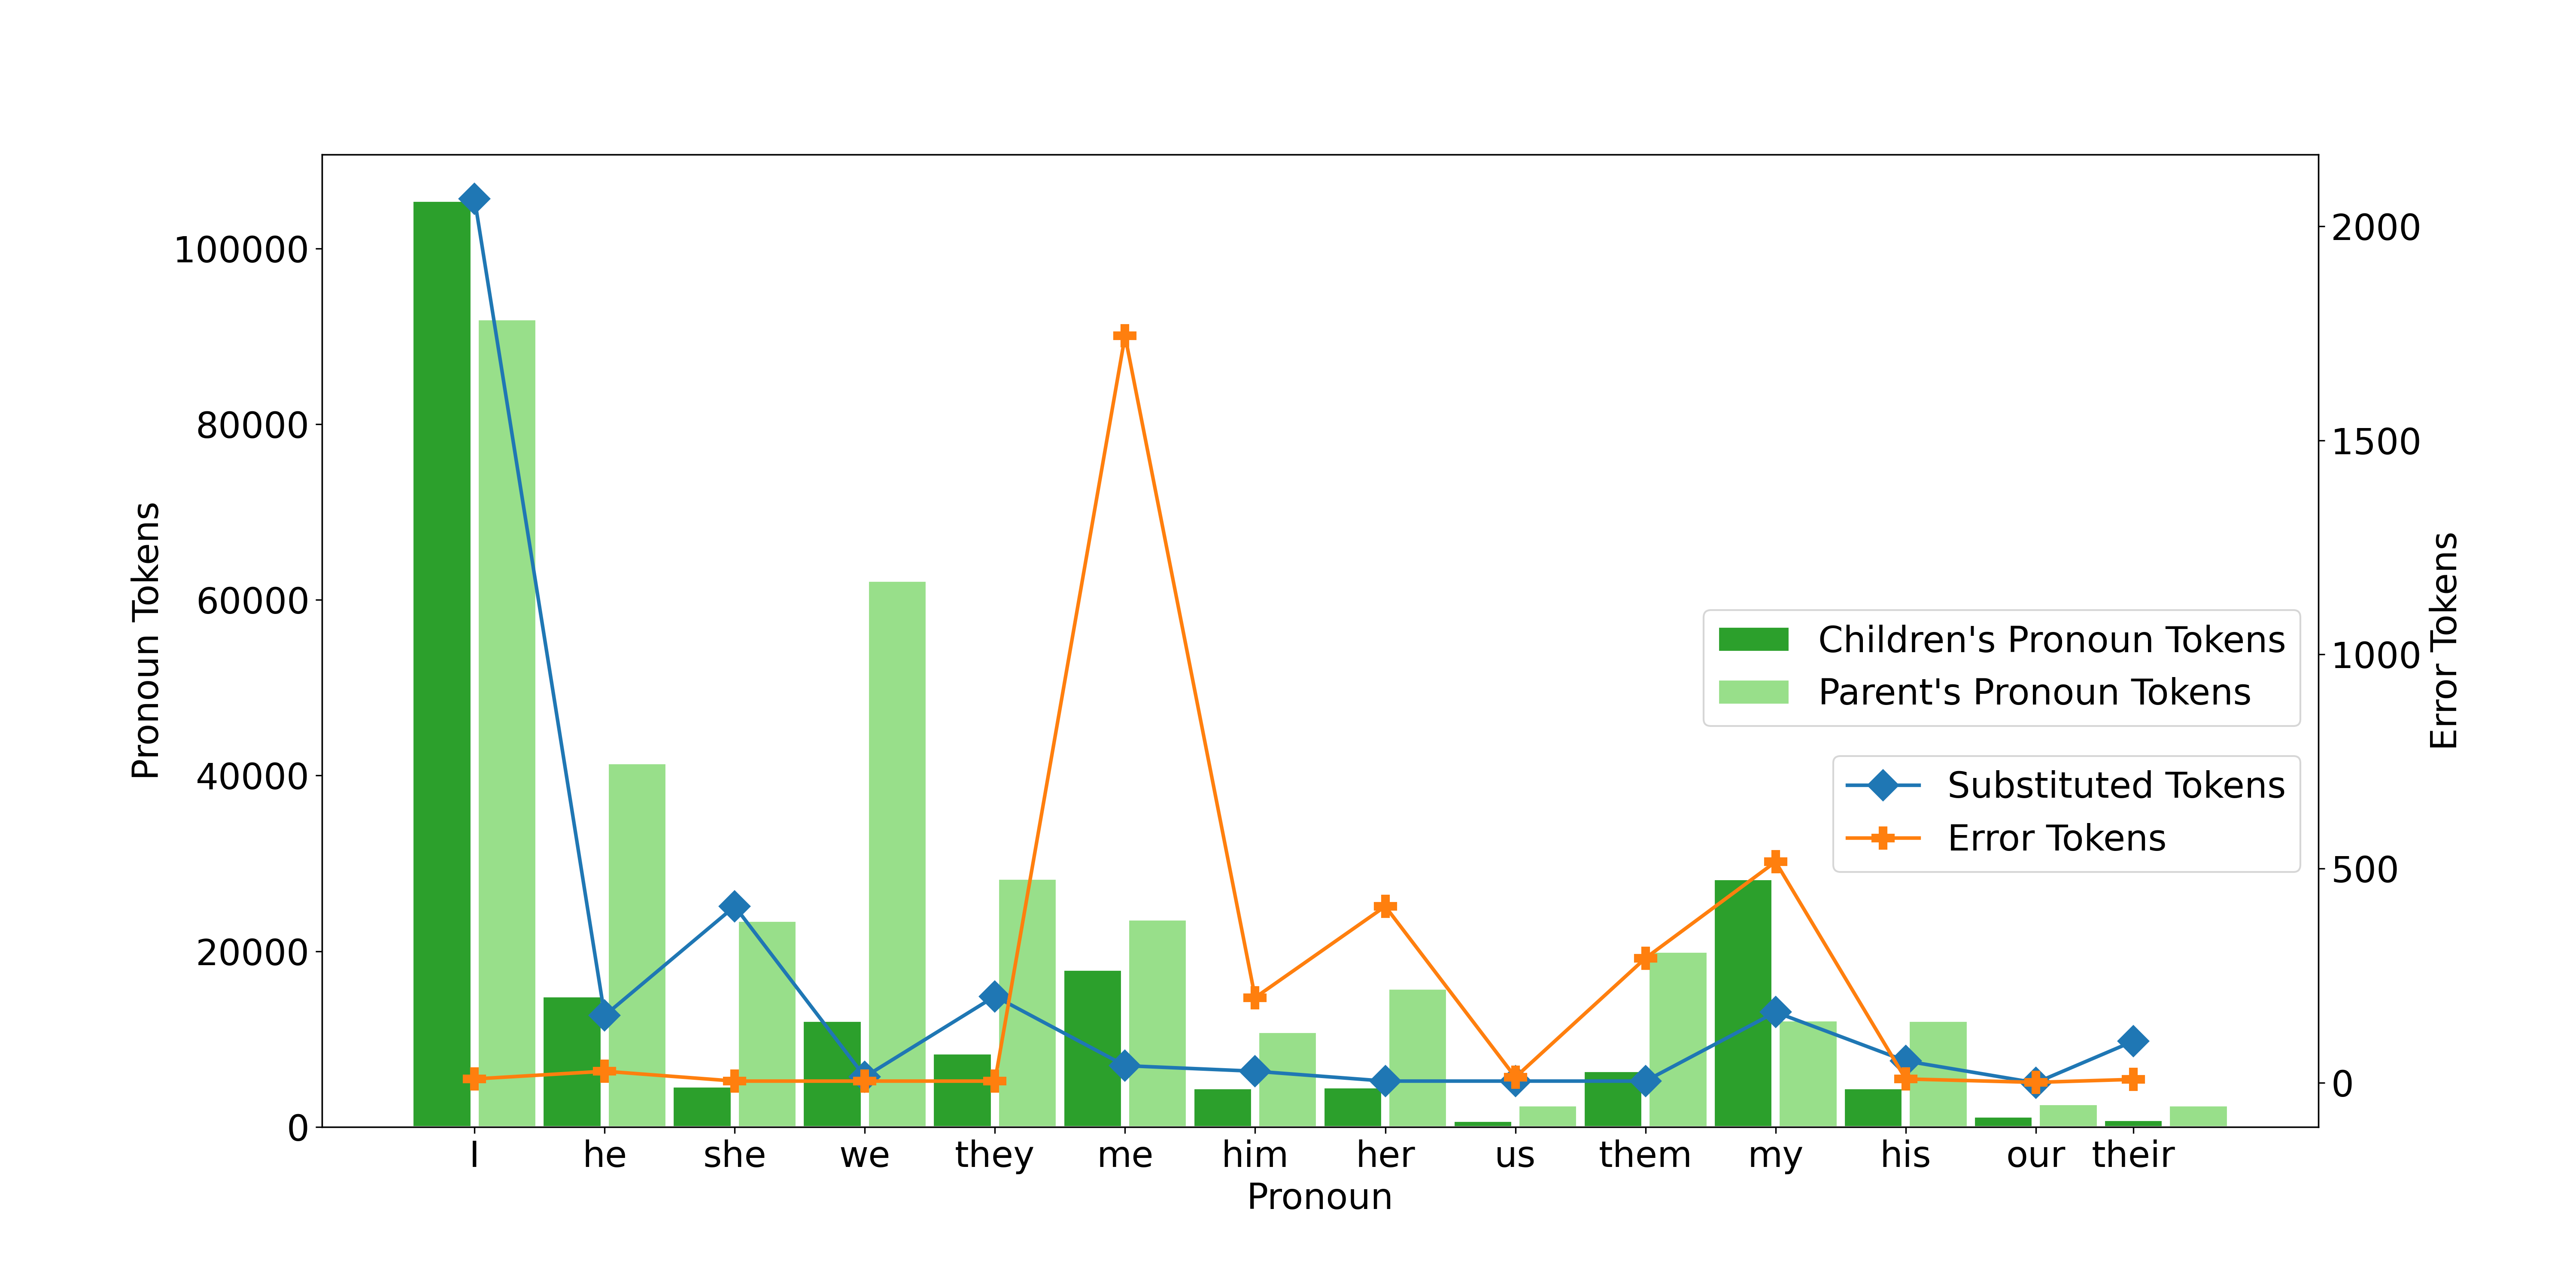
\includegraphics[scale = 0.35]{graph/Pronounandtoken.png}
    \vspace{-2em}
    \caption{Error tokens and Substituted tokens and Pronoun tokens by Parents and Children}
    \label{fig:errortoken}
\end{figure}
\FloatBarrier


\subsection{Conclusion}
This section analyzed pronoun case error's frequency and pattern. First, pronoun case error is a relatively uncommon phenomenon, that most of the children rarely make any errors. 141 children in the cross-sectional data didn't make any errors, and 32 children with longitudinal recordings have less than 1\% of error rate. The average pronoun case error rate is also extremely low, with an average 1.16\% error rate for the cross-sectional data and 1.56\% for the longitudinal data. 

The pronoun case error rate has a non-monotonic relationship with children's age and mlu. The pronoun correct rate displays a U-shaped developmental pattern that children start with almost 100\% correct rate and decline to around 97\% and rise back to almost 100\% at around 5 years old. However, the correct rate at different age groups are not significantly different from each other. Since the error rate is so low during the U-shaped developmental sequences, it is difficult to judge if the changes in the correct rate are meaningful. 

Children's pronoun production and parents' pronoun input are not correlated with pronoun correr rate or pronoun error tokens. The substituted tokens are correlated with children's pronoun production, suggesting that the more children use a pronoun, the more often that pronoun is to be substituted by an incorrect pronoun. 

\section{Study 2. Can Children's Verbal Use Explain Pronoun Case Errors?}
(Replicating ATOM model)
\section{Study 3. Can Parents' Input Explain Pronoun Case Errors?}
(Replicating \cite{kirjavainen2009can})
\section{Study 4. Do Children Have a Pronoun Paradigm?}
(Replication Rispli)
\section{Study 5. A Computational Model of Children's Pronoun Acquisition}